\documentclass{llncs}

\usepackage[ngerman]{babel}
\usepackage[utf8]{inputenc} % latin1 anstatt utf8 falls Umlaute defekt
\usepackage{graphicx}
\graphicspath{{img/}}
\usepackage{pdfsync}
\usepackage{float}
\usepackage{amssymb}
\usepackage{amsmath}
\usepackage{tikz}

\newtheorem{satz}{Satz}{}

\renewcommand{\labelitemi}{$\bullet$}

%\DeclareUnicodeCharacter{00A0}{ }

\begin{document}
\title{Verteiltes Wissen}
\subtitle{\small{ Seminar Modellierung verteilter Systeme (MvS)\\ Sommersemester 2016,}}
\author{Danny Schubert, Jan Fabian Schmid\\\email{\{5schuber,2schmid\}@informatik.uni-hamburg.de}}
\institute{Universität Hamburg}
\maketitle

\begin{abstract}
In einem verteilten System müssen die Prozesse sinnvolle Entscheidungen mit unvollständigen Wissen über das Gesamtsystem fällen.
Diese Seminar-Arbeit behandelt die Frage, wie Prozesse mit dem Wissen, das ihnen zur Verfügung steht, mittels logischer Schlussfolgerungen Informationen ableiten können.
Dazu wird eine formale Logik mit intuitiver Repräsentation vorgestellt.
Es zeigt sich, dass es eine große Rolle spielt, wie ein Prozess eine neue Information erhalten hat, also wie das Nachrichtensystem funktioniert. Das liegt daran, dass ein Prozess je nach Nachrichtensystem unterschiedliche Annahmen an das Wissen anderer Prozesse machen kann.
Das Problem, das durch asynchrone Nachrichtensysteme entsteht, kann auf das Konsens-Problem zurückgeführt werden.
Dieses Problem kann durch schwächere Forderungen an das Wissen in verteilten Systemen umgangen werden.
Am Ende der Arbeit wird noch deutlich gemacht, dass es nicht zu unterschätzen ist, wie viel einfacher Lösungen zu einem Problem gefunden werden können, wenn die Prozesse des Systems größere Freiheiten bei der Kommunikation miteinander haben.
\end{abstract}

\section{Einleitung}
Im Gegensatz zu einem einfachen zentralisierten System müssen in einem verteilten System Entscheidungen auf Grundlage unvollständiger Informationen getroffen werden.
Die einzelnen Prozesse des verteilten Systems können nicht ohne Einschränkungen Kenntnis über die Zustände der anderen Prozesse erlangen.
So muss der Informationsaustausch zweier Prozesse mit Hilfe von Nachrichten durchgeführt werden. Diese Nachrichten haben eine endliche, oft unbekannte, Laufzeit.
Entscheidungen eines Prozesses müssen daher mit den unvollständigen, veralteten oder schlicht falschen lokalen Informationen über das Gesamtsystem getroffen werden.\\
In dieser Arbeit soll betrachtet werden wie lokale Prozesse mit Hilfe von Wissenslogik Informationen über das System ableiten und unter welchen Umständen sie korrekte Entscheidungen treffen können.

\subsection{Motivation: Das \textit{cheating husbands}-Rätsel}
Um das Konzept von verteiltem Wissen zu veranschaulichen nutzen Moses et al. \cite{moses1986cheating} das \textit{cheating husbands}-Rätsel (vgl. \cite{moses1986cheating} S. 168 ff.).
Dabei handelt es sich um ein Induktions-Rätsel von dem es viele Varianten gibt (\textit{unfaithful wives problem}, \textit{blue eyes problem}, \textit{muddy children puzzle}). Auch wir werden dieses Beispiel als durchgehende Veranschaulichung der Theorie verwenden.\\
Das Rätsel wird im Rahmen einer Geschichte aufgestellt: Die Königin Henrietta I von Atlantis möchte das Untreue-Problem in der Stadt Mamajorca lösen unter dem die Frauen leiden.
Folgende Informationen können als gemeinsames Wissen unter der Bevölkerung der Stadt vorausgesetzt werden:
\begin{itemize}
	\item Die Königin sagt die Wahrheit.
	\item Alle Ehefrauen gehorchen der Königin.
	\item Die Ehefrauen sind perfekte Logiker.
	\item Ein Pistolenschuss kann in der ganzen Stadt gehört werden.
	\item Keine Ehefrau weiß, ob ihr Ehegatte sie betrügt.
	\item Jede Ehefrau weiß welche der anderen Frauen betrogen worden sind.
\end{itemize}
Um das Untreue-Problem zu lösen lässt Henrietta I alle Ehefrauen der Stadt zusammenkommen und verkündet dann vor ihnen, dass es mindestens einen untreuen Ehemann gibt ($n \ge 1$).
Die Königin verbietet (aufgrund der Etikette), dass die Ehefrauen miteinander über die untreuen Ehemänner reden.
Sollte eine Ehefrau jedoch herausfinden, dass ihr Gatte untreu war, so muss sie ihn am selben Tag um Mitternacht erschießen.\medskip

Folgendes kann gezeigt werden:\\
Wenn es $n$ untreue Ehemänner zum Zeitpunkt der Verkündung von Henrietta I gab, so werden diese alle um Mitternacht des n-ten folgenden Tages (einschließlich des Tages der Verkündigung) erschossen.\medskip

Beweis mittels vollständiger Induktion über die Anzahl der untreuen Ehemänner:\\
\textbf{Induktionsanfang:} Angenommen es gäbe einen ($n=1$) untreuen Ehemann. So gäbe es eine Ehefrau, die keine andere Ehefrau kennen würde, die betrogen wurde. Da es mindestens einen untreuen Ehemann gibt kann sie darauf schließen, dass es ihr Mann sein muss. Dementsprechend wird der eine untreue Ehemann noch am selben Tag (also am ersten folgenden Tag nach der Verkündigung) um Mitternacht erschossen.\\
\textbf{Induktionsvoraussetzung:} Die Behauptung gelte für den Fall mit $n$ untreuen Ehemännern.\\
\textbf{Induktionsschluss:} Gezeigt werden muss nun, dass die Behauptung auch für $n+1$ untreue Ehemänner gilt.
Jede betrogene Ehefrau weiß in diesem Fall von $n$ betrogenen Ehefrauen in der Stadt. Die nicht betrogenen Ehefrauen hingegen kennen alle $n+1$ betrogenen Ehefrauen.
Aufgrund der Induktionsvoraussetzung wissen die betrogenen Ehefrauen, dass alle ihr bekannten betrogenen Ehefrauen ihre Männer in der n-ten Nacht erschossen hätten, wenn es tatsächlich nur $n$ untreue Ehemänner gibt.
Da dies nicht geschehen ist, wissen die betrogenen Ehefrauen, dass es $n+1$ untreue Ehemänner geben muss und das ihrer einer davon ist.
Die betrogenen Ehefrauen mussten dementsprechend darauf warten, ob in der n-ten Nacht Schüsse zu  hören sind, um zu entscheiden, ob sie ihren Ehemann erschießen müssen.
Nach der n-ten Nacht weiß jede betrogene Ehefrau, dass ihr Mann sie betrogen hat, sodass alle untreuen Ehemänner in der n+1-ten Nacht um Mitternacht erschossen werden. $\square$

Entscheidend bei diesem Szenario ist, dass die Königin die Information, dass es mindestens einen untreuen Ehemann gibt, zu gemeinsamen Wissen macht.
Ohne dieses Wissen gilt der Induktionsanfang nicht; tatsächlich werden die Ehefrauen nie herausfinden, ob ihr Ehemann untreu war, wenn diese Information nicht allgemein bekannt gemacht wird (vgl. \cite{kshemkalyani2011distributed} S.283).

\subsection{Probleme und Fragen}
Eines der zentralen Probleme besteht in der Unmöglichkeit gemeinsames Wissen mehrerer Prozesse in einem asynchronen System herzustellen, wenn die Prozesse fehlerhaft handeln können (vgl.\cite{kshemkalyani2011distributed} S. 293 f.). Um mit asynchronen Systemen in der Praxis arbeiten zu können, nutzt man daher Verfahren die eingeschränktes gemeinsames Wissen ermöglichen.\\
Weitere Fragestellungen des Themas untersuchen wie die Art des Nachrichtensystems das Wissen der lokalen Prozesse beeinflusst und wie die Informationsbeziehungen zwischen den Prozessen visuell dargestellt werden können.

\subsection{Aufbau der Arbeit}
Im Kapitel \ref{Logik} werden zunächst die Logikoperatoren eingeführt, mit denen in verteilten System Wissen abgeleitet werden kann.
Um die Beziehungen zwischen den Prozessen und die Entwicklung von Wissen in verteilten Systemen intuitiv darzustellen, werden in Kapitel \ref{Kripke-Modelle} Kripke-Modelle genutzt. Kapitel \ref{sync_vs_async} geht der Frage nach, wie das ableitbare Wissen in einem System davon abhängt, ob das Nachrichtensystem synchron oder asynchron funktioniert. Um das Konsens-Problem zu vermeiden werden in Kapitel \ref{GemeinsamesWissen} schwächere Definitionen von gemeinsamen Wissen vorgestellt.
Abschließend wird die Arbeit in Kapitel \ref{Zusammenfassung} zusammengefasst.
\section{Logik des Wissens}
\label{Logik}
Damit möglichst intuitiv Logik über das Wissen in verteilten Systemen betrieben werden kann, werden Logikoperatoren aus der epistemischen Logik genutzt, mit denen eine Logik (bspw. Aussagenlogik) erweitert werden kann.

Fagin et al. führen dazu zunächst das Konzept von \textbf{möglichen Welten} ein (vgl. \cite{fagin2003reasoning} S.15 ff.). 
Da ein einzelner Prozess in einem verteilten System nur eingeschränkte Informationen über die Zustände in den anderen Prozessen hat, kann es verschiedene Systemzustände geben, die er anhand seiner lokalen Informationen bzw. Zustände nicht voneinander unterscheiden kann. Die möglichen Welten $P_i$ werden daher definiert als: Die Vereinigung aller Systemzustände, die mit den vorhanden Informationen eines Prozesses $i$ vereinbar sind.
Mit Hilfe der möglichen Welten können Aussagen über eine Formel $\phi$ gemacht werden:
Ein Prozess $i$ \textit{weiß}, dass $\phi$ gilt ($K_i\phi$), wenn in allen Welten, die er für möglich hält, $\phi$ gilt.
%Die Syntax zur Wissenslogik kann entsprechend ausgedrückt werden als:
%\begin{align*}
%\phi &::= p | \neg\phi_1 | \phi_1 \land \phi_2 | K_i\phi
%\end{align*}
%Wobei $p\in P$ eine atomare Aussagenlogische Formel ist, $\phi_1$ und $\phi_2$ sind Formeln unserer Wissenslogik und $i \in \{1,...,n\}$ in einem verteilten System mit $n$ Prozessen.
Die Semantik zu den Logikoperatoren des Wissens kann mit Hilfe von \textbf{Kripke-Modellen} definiert werden (vgl. \cite{kshemkalyani2011distributed} S. 285 f.).
Ein Kripke-Modell $M$ zu einem verteilten System mit $n$ Prozessen und einer Menge atomarer Aussagen $\Phi$ ist ein Tupel $(S,\pi,\mathcal{K}_1,...,\mathcal{K}_n)$ mit der Menge möglicher Systemzustände $S$, der Belegungsfunktion $\pi$, die jeder atomaren Aussage in jedem Zustand $s$ einen Wahrheitswert zuordnet ($\forall s\in S, \pi(s):\Phi \rightarrow \{0,1\}$) und einer binären Relation $\mathcal{K}_i$ auf $S$ für jeden Prozess $i$, die jedem Prozess $i$ seine möglichen Welten, also die Menge von Systemzuständen die er nicht vom tatsächlichen Systemzustand unterscheiden kann, zuordnet. $\mathcal{K}_i$ enthält für alle Zustände $s \in S$ alle Tupel ($s,t$) von Zuständen die anhand seiner lokalen Informationen nicht unterscheidbar sind. \medskip

Damit ergeben sich folgende Definitionen der Wissensoperatoren:
\begin{itemize}
\item (M,s) $\vDash \phi$, falls $\pi(s)(\phi) = true$
\item (M,s) $\vDash K_i(\phi)$, falls für alle t $\in S$ mit $(s,t) \in \mathcal{K}_i $ gilt: (M,t) $\vDash \phi$
\item (M,s) $\vDash E^1(\phi)$, falls (M,s) $\vDash\land_{i\in N}K_i(\phi)$
\item (M,s) $\vDash E^{k+1}(\phi)$ mit $k\ge 1$, falls (M,s) $\vDash\land_{i\in N}K_i(E^k(\phi))$
\item (M,s) $\vDash C(\phi)$, falls (M,s) $\vDash\land_{k\in Z^*}E^k(\phi)$
\end{itemize}

Dabei ist K der bereits erwähnte Wissensoperator, E der \textit{jeder weiß}-Operator und C der \textit{gemeinsames Wissen}-Operator.
Der \textit{jeder weiß}-Operator wird rekursiv für höhere Ebenen definiert: $E^1(\phi)$ bedeutet, dass jeder Prozess im System weiß, dass $\phi$ gilt; $E^2(\phi)$ bedeutet, dass jeder Prozess weiß, dass jeder Prozess weiß, dass $\phi$ gilt, und so weiter.
Der \textit{gemeinsames Wissen}-Operator kann intuitiv so verstanden werden, dass es definitiv für keinen Prozess einen Zweifel daran gibt, dass den anderen Prozessen $\phi$ bekannt ist. Dies gilt beispielsweise in unserer ersten Version des \textit{cheating husbands}-Rätsels für die Information, dass es mindestens einen untreuen Ehemann gibt, nachdem die Königin dies in der Gegenwart aller Ehefrauen verkündet hat. 
\section{Veranschaulichung mit Kripke-Modellen}
\label{Kripke-Modelle}
Das Kripke-Modell eines verteilten Systems mit kleiner Anzahl Prozesse kann intuitiv als Graph dargestellt werden (vgl. \cite{kshemkalyani2011distributed} S. 285 ff.).
Dazu wird ein Graph gezeichnet, dessen Bestandteile den Objekten des Kripke-Modell Tupels entsprechen.
Jeder Systemzustand $s\in S$ entspricht einem Knoten, der mit der Belegung von $\pi$ für die atomaren Aussagen $\Phi$ beschriftet wird. Eine Kante wird zwischen zwei Knoten gezeichnet, wenn es mindestens einen Prozess gibt, der die repräsentierten Systemzustände nicht voneinander unterscheiden kann. Sie wird mit den Nummern aller Prozesse beschriftet für die dies gilt.
Der Graph ist dementsprechend bidirektional und reflexiv.\\
Mit Hilfe der Erreichbarkeit können die Definitionen zu den \textit{jeder-weiß}- und den \textit{gemeinsames Wissen}-Operator auf diese Graphen übertragen werden:
\begin{itemize}
	\item Ein Zustand t kann vom Zustand s in k Schritten erreicht werden (ist k-erreichbar), wenn es eine Folge von Zuständen $s_0,s_1,...,s_k$ gibt, wobei $s_0 = s$, $s_k = t$ mit einem Zustand $P_i$ zu jedem $j\in [ 0,k-1 ]$, sodass $(s_j,s_{j+1})\in \mathcal{K}_i$
	\item Ein Zustand t ist vom Zustand s aus erreichbar, wenn es ein beliebiges $k \ge 0$\footnote{\label{note1}In \cite{kshemkalyani2011distributed} S. 286 wird dies für ein $k > 1$ definiert. Zum Ende dieses Kapitels wird auf den Unterschied der beiden Definitionen eingegangen.} gibt, sodass t von s in k Schritten erreicht werden kann.
\end{itemize}
Man kann also direkt am Graphen erkennen, welche Zustände von einem anderen k-erreichbar sind, indem man alle Wege verfolgt, die sich mit k Kanten bilden lassen.
Generell erreichbar ist ein Zustand, wenn es eine ununterbrochene Verbindung zu ihm gibt.
Daraus ergeben sich für den \textit{jeder-weiß}- und den \textit{gemeinsames Wissen}-Operator folgende Definitionen:
\begin{itemize}
	\item (M,s) $\vDash E^{k}(\phi)$, genau dann wenn (M,t) $\vDash \phi$ für alle Zustände t gilt, die vom Zustand s in k (oder weniger)\footnote{\label{note2}In \cite{kshemkalyani2011distributed} S. 286 fehlt dieser Zusatz. Zum Ende des Kapitels wird auf den Unterschied eingegangen.} Schritten erreichbar sind.
	\item (M,s) $\vDash C(\phi)$, genau dann wenn (M,t) $\vDash \phi$ für alle Zustände t gilt, die vom Zustand s erreichbar sind.
\end{itemize}
Um im Graphen zu erkennen, ob $E^{k}(\phi)$ in einem Zustand s gilt, muss man dementsprechend überprüfen, ob $\phi$ in allen Zuständen wahr ist, die sich in k oder weniger Schritten erreichen lassen. 
Warum diese Definitionen für den \textit{jeder-weiß}- und den \textit{gemeinsames Wissen}-Operator mit denen aus dem vorherigen Kapitel übereinstimmen werden wir anhand mehrerer Beispiele im Folgenden erkennen.

\subsection{Kripke-Modelle zum \textit{cheating husbands}-Rätsel}
Die aufgestellten Definitionen können mit Hilfe des \textit{cheating husbands}-Rätsels veranschaulicht werden.
Für den Fall, dass es drei Ehepaare in Atlantis gibt, lässt sich die Situation noch dreidimensional darstellen.
In Abbildung \ref{ausgang} betrachten wir zunächst die Ausgangssituation noch bevor die Königin ihre Ansprache auf dem Marktplatz gehalten hat.
Ein Zustand (0,0,1) im Graphen bedeutet, dass der Ehemann des dritten Ehepaares untreu war, während die anderen beiden treu sind.

\begin{figure}
\centering
\begin{tikzpicture}[thick,scale=0.2]
\coordinate[label={180:\text{(1,0,0)}}] (UVL) at (0,0,12);
\coordinate[label={0:\text{(1,1,0)}}] (UVR) at (12,0,12);
\coordinate[label={180:\text{(0,0,0)}}] (OVL) at (0,12,12);
\coordinate[label={-120:\text{(0,1,0)}}] (OVR) at (12,12,12);
\coordinate[label={-86:\text{(1,0,1)}}] (UHL) at (0,0,0);
\coordinate[label={0:\text{(1,1,1)}}] (UHR) at (12,0,0);
\coordinate[label={180:\text{(0,0,1)}}] (OHL) at (0,12,0);
\coordinate[label={0:\text{(0,1,1)}}] (OHR) at (12,12,0);

\draw[fill=black] (UVL) circle (8pt);
\draw[fill=black] (UVR) circle (8pt);
\draw[fill=black] (OVL) circle (8pt);
\draw[fill=black] (OVR) circle (8pt);
\draw[fill=black] (UHL) circle (8pt);
\draw[fill=black] (UHR) circle (8pt);
\draw[fill=black] (OHL) circle (8pt);
\filldraw[color=black] (OHR) circle (8pt);

\draw (UVL) -- node[above] {2} (UVR);
\draw (UVL) -- node[above left] {1} (OVL);
\draw (UVL) -- node[left] {3} (UHL);
\draw (OVR) -- node[above right] {2} (OVL);
\draw (OVR) -- node[left] {3} (OHR);
\draw (OVR) -- node[above left] {1} (UVR);
\draw (OHL) -- node[left] {3} (OVL);
\draw (OHL) -- node[above] {2} (OHR);
\draw (OHL) -- node[left] {1} (UHL);
\draw (UHR) -- node[left] {3} (UVR);
\draw (UHR) -- node[left] {1} (OHR);
\draw (UHR) -- node[above left] {2} (UHL);
\end{tikzpicture}
\caption{Ausgangssituation des \textit{cheating husbands}-Rätsels}
\label{ausgang}
\end{figure}

In der graphischen Darstellung kann man gut die Symmetrie des Problems erkennen.
Die i-te Ehefrau kann die Zustände nicht unterscheiden, dessen Werte nur an der i-ten Stelle variieren.
So kann beispielsweise die erste Ehefrau die Situationen (0,0,0) und (1,0,0) nicht voneinander unterscheiden, da sie nicht weiß, ob ihr eigener Ehemann untreu war. Gleiches gilt für die Zustände (0,0,1) zu (1,0,1), (0,1,0) zu (1,1,0) und (0,1,1) zu (1,1,1).\medskip

Gehen wir nun davon aus, dass der zweite und dritte Ehemann untreu waren und wir uns somit im Zustand (0,1,1) befinden.
Nachdem die Königin ihre Ansprache gehalten hat, verändert sich die Kripke-Struktur, wie in Abbildung \ref{nachAnsprache} gezeigt.

\begin{figure}
	\centering
	\begin{tikzpicture}[thick,scale=0.2]
	\coordinate[label={180:\text{(1,0,0)}}] (UVL) at (0,0,12);
	\coordinate[label={0:\text{(1,1,0)}}] (UVR) at (12,0,12);
	\coordinate[label={180:\text{(0,0,0)}}] (OVL) at (0,12,12);
	\coordinate[label={-120:\text{(0,1,0)}}] (OVR) at (12,12,12);
	\coordinate[label={-86:\text{(1,0,1)}}] (UHL) at (0,0,0);
	\coordinate[label={0:\text{(1,1,1)}}] (UHR) at (12,0,0);
	\coordinate[label={180:\text{(0,0,1)}}] (OHL) at (0,12,0);
	\coordinate[label={0:\text{(0,1,1)}}] (OHR) at (12,12,0);
	
	\draw[fill=black] (UVL) circle (8pt);
	\draw[fill=black] (UVR) circle (8pt);
	\draw[fill=black] (OVL) circle (8pt);
	\draw[fill=black] (OVR) circle (8pt);
	\draw[fill=black] (UHL) circle (8pt);
	\draw[fill=black] (UHR) circle (8pt);
	\draw[fill=black] (OHL) circle (8pt);
	\filldraw[color=red] (OHR) circle (8pt);
	
	\draw (UVL) -- node[above] {2} (UVR);

	\draw (UVL) -- node[left] {3} (UHL);

	\draw (OVR) -- node[left] {3} (OHR);
	\draw (OVR) -- node[above left] {1} (UVR);
	
	\draw (OHL) -- node[above] {2} (OHR);
	\draw (OHL) -- node[left] {1} (UHL);
	\draw (UHR) -- node[left] {3} (UVR);
	\draw (UHR) -- node[left] {1} (OHR);
	\draw (UHR) -- node[above left] {2} (UHL);
	\end{tikzpicture}
	\caption{Kripke-Modell nach der Ansprache der Königin.}
	\label{nachAnsprache}
\end{figure}

Da es nach der Ansprache das gemeinsame Wissen gibt, dass es mindestens einen untreuen Ehemann in Atlantis gibt, kann der Zustand (0,0,0) von allen Ehefrauen ausgeschlossen werden. Alle Kanten zu (0,0,0) werden dementsprechend entfernt.
Der entscheidende Unterschied zur Ausgangssituation besteht darin, dass es nun Zustände gibt, die von einzelnen Ehefrauen eindeutig identifiziert werden können. Es gibt also Zustände von denen nicht für jeden Prozess eine Kante ausgeht. Dies sind derzeit alle Zustände in denen nur ein Ehemann untreu war.
Der Induktions-Anfang aus Kapitel \ref{motivation} nutzt gerade diese Eigenschaft aus. Wenn es $n=1$ untreue Ehemänner gibt, so kennt dessen Ehefrau keinen untreuen Ehemann und induziert daher, dass ihr eigener Ehemann untreu gewesen sein muss. Diese Situation kann die betroffene Ehefrau mit keiner anderen verwechseln.\\
Da jede Ehefrau in unserem Fall mindestens einen untreuen Ehemann kennt, geschieht in der ersten Nacht nichts. Am nächsten Tag ergibt sich dann die Situation aus Abbildung \ref{zweiterTag}.

\begin{figure}
	\centering
	\begin{tikzpicture}[thick,scale=0.2]
	\coordinate[label={180:\text{(1,0,0)}}] (UVL) at (0,0,12);
	\coordinate[label={0:\text{(1,1,0)}}] (UVR) at (12,0,12);
	\coordinate[label={180:\text{(0,0,0)}}] (OVL) at (0,12,12);
	\coordinate[label={-120:\text{(0,1,0)}}] (OVR) at (12,12,12);
	\coordinate[label={-86:\text{(1,0,1)}}] (UHL) at (0,0,0);
	\coordinate[label={0:\text{(1,1,1)}}] (UHR) at (12,0,0);
	\coordinate[label={180:\text{(0,0,1)}}] (OHL) at (0,12,0);
	\coordinate[label={0:\text{(0,1,1)}}] (OHR) at (12,12,0);
	
	\draw[fill=black] (UVL) circle (8pt);
	\draw[fill=black] (UVR) circle (8pt);
	\draw[fill=black] (OVL) circle (8pt);
	\draw[fill=black] (OVR) circle (8pt);
	\draw[fill=black] (UHL) circle (8pt);
	\draw[fill=black] (UHR) circle (8pt);
	\draw[fill=black] (OHL) circle (8pt);
	\filldraw[color=red] (OHR) circle (8pt);	
	
	\draw (UHR) -- node[left] {3} (UVR);
	\draw (UHR) -- node[left] {1} (OHR);
	\draw (UHR) -- node[above left] {2} (UHL);

	\end{tikzpicture}
	\caption{Kripke-Modell nach der ersten Nacht.}
	\label{zweiterTag}
\end{figure}

Da in der ersten Nacht kein Schuss zu hören war, ist es nun gemeinsames Wissen, dass es mindestens zwei untreue Ehemänner gibt.
Die zweite und dritte Ehefrau wissen nur von einem untreuen Ehemann und können somit schlussfolgern, dass sie selbst betrogen wurden. Da sie wissen, welche der anderen Ehefrauen betrogen wurden sind wissen sogar, dass (0,1,1), der wahre Systemzustand ist. Beide Ehefrauen erschießen ihren Ehemann, sodass am nächsten Tag auch die erste Ehefrau den korrekten Zustand kennt.

\subsubsection{Visualisierung der Wissensoperatoren}
Um die Äquivalenz der Definitionen für den \textit{jeder weiß}- und den \textit{gemeinsames Wissen}-Operator aufzuzeigen, betrachten wir noch einmal die Ausgangssituation des \textit{cheating husbands}-Rätsels. 
Die Formel $\Phi$ beschreibe die Eigenschaft, dass es mindestens einen untreuen Ehemann gibt.
In der Ausgangssituation wurde $\Phi$ noch nicht von der Königin bekannt gemacht.
Warum ist $\Phi$ ausgehend vom tatsächlichen Zustand (0,1,1) kein gemeinsames Wissen?\\
Damit $C(\Phi)$ gilt, muss nach der ursprünglichen Definition $E^k(\Phi)$ für alle $k>0$ gelten.
Da jede Ehefrau in diesem Zustand mindestens von einem untreuen Ehemann weiß gilt $E^1(\Phi)$.
Zwei der drei Ehefrauen wissen nur von einem untreuen Ehemann, sie halten die Welt für möglich, in der dieser Ehemann der einzige untreue war.
Ausgehend von so einer Welt, denken die beiden Ehefrauen weiter, würde die einzige betrogene Ehefrau von keinem untreuen Ehemann wissen.
Im Zustand (0,1,1) weiß somit beispielsweise die dritte Ehefrau nicht, ob die zweite Ehefrau weiß, dass es mindestens einen untreuen Ehemann gibt.
Obwohl jede Ehefrau weiß, dass es mindestens einen untreuen Ehemann gibt, ist diese Information kein gemeinsames Wissen.
Somit gilt in der Ausgangssituation nicht $C(\Phi)$, der Induktionsanfang aus \ref{motivation} greift somit nicht, und es kann nie ein Ehemann erschossen werden.\\

Diese Überlegungen können mit Hilfe der Definitionen zu den \textit{jeder weiß}- und den gemeinsames Wissen-Operator, die k-Erreichbarkeit ausnutzen, leicht am Graphen verifiziert werden.
In jedem Zustand der von (0,1,1) in einem oder keinem Schritt erreichbar ist, gibt es mindestens einen untreuen Ehemann. In zwei Schritten ist allerdings (0,0,0) erreichbar. Somit gilt $E^1(\Phi)$, nicht aber $E^2(\Phi)$, also auch nicht $C(\Phi)$.\medskip

An dieser Stelle können wir kurz betrachten, warum die Zusätze $^1$ und $^2$ zu den Definitionen von \cite{kshemkalyani2011distributed} sinnvoll sind:
\begin{itemize}
	\item Wird (M,s) $\vDash E^{k}(\phi)$ ohne den Zusatz \glqq oder weniger\grqq{} definiert, könnte man denken, dass im Zustand (0,0,0) $E^1(\Phi)$ gilt, denn in allen Zuständen, die in genau einem Schritt erreichbar sind, gilt $\Phi$. Diese Eigenschaft gilt allerdings offensichtlich nicht, denn jede der drei Ehefrauen hält in diesem Zustand auch den Zustand (0,0,0) selbst für möglich und ihn diesem gibt es keinen einzigen untreuen Ehemann.
	Technisch gesehen ist (0,0,0) auch in einem Schritt von (0,0,0) erreichbar, denn es existiert eine Folge von Zuständen $s_0$ und $s_1$, wobei $s_0$ = (0,0,0) und $s_1$ = (0,0,0), die für jedes $P_i$ in $\mathcal{K}_i$ enthalten sind.
	Somit ist die Definition aus der Literatur korrekt. Mit dem von uns eingefügten Zusatz wird diese allerdings intuitiver verständlich.
	\item Wird die generelle Erreichbarkeit mit $k > 1$, also $k \ge 2$, statt $k \ge 0$ definiert, gibt es ebenso Situationen in denen unintuitive Zustandsfolgen mit dem selben Zustand genutzt werden müssen, um die Eigenschaften aufzuzeigen.
	So muss in einem Kripke-Modell, in dem nur der Zustand (0,0,0) existiert, die Folge (0,0,0),(0,0,0),(0,0,0) betrachtet werden, wenn man zeigen möchte, dass $\Phi$ nicht gilt. Mit unserer Definition kann direkt aus (0,0,0) geschlossen werden, dass $\Phi$ in diesem Kripke-Modell nicht gilt.
\end{itemize}
%########################################################################################
% Chapter: Wissen in synchronen und asynchronen Systemen
%########################################################################################
\section{Wissen in synchronen und asynchronen Systemen}
\label{sync_vs_async}
%\begin{figure}[H]
%\centering
%      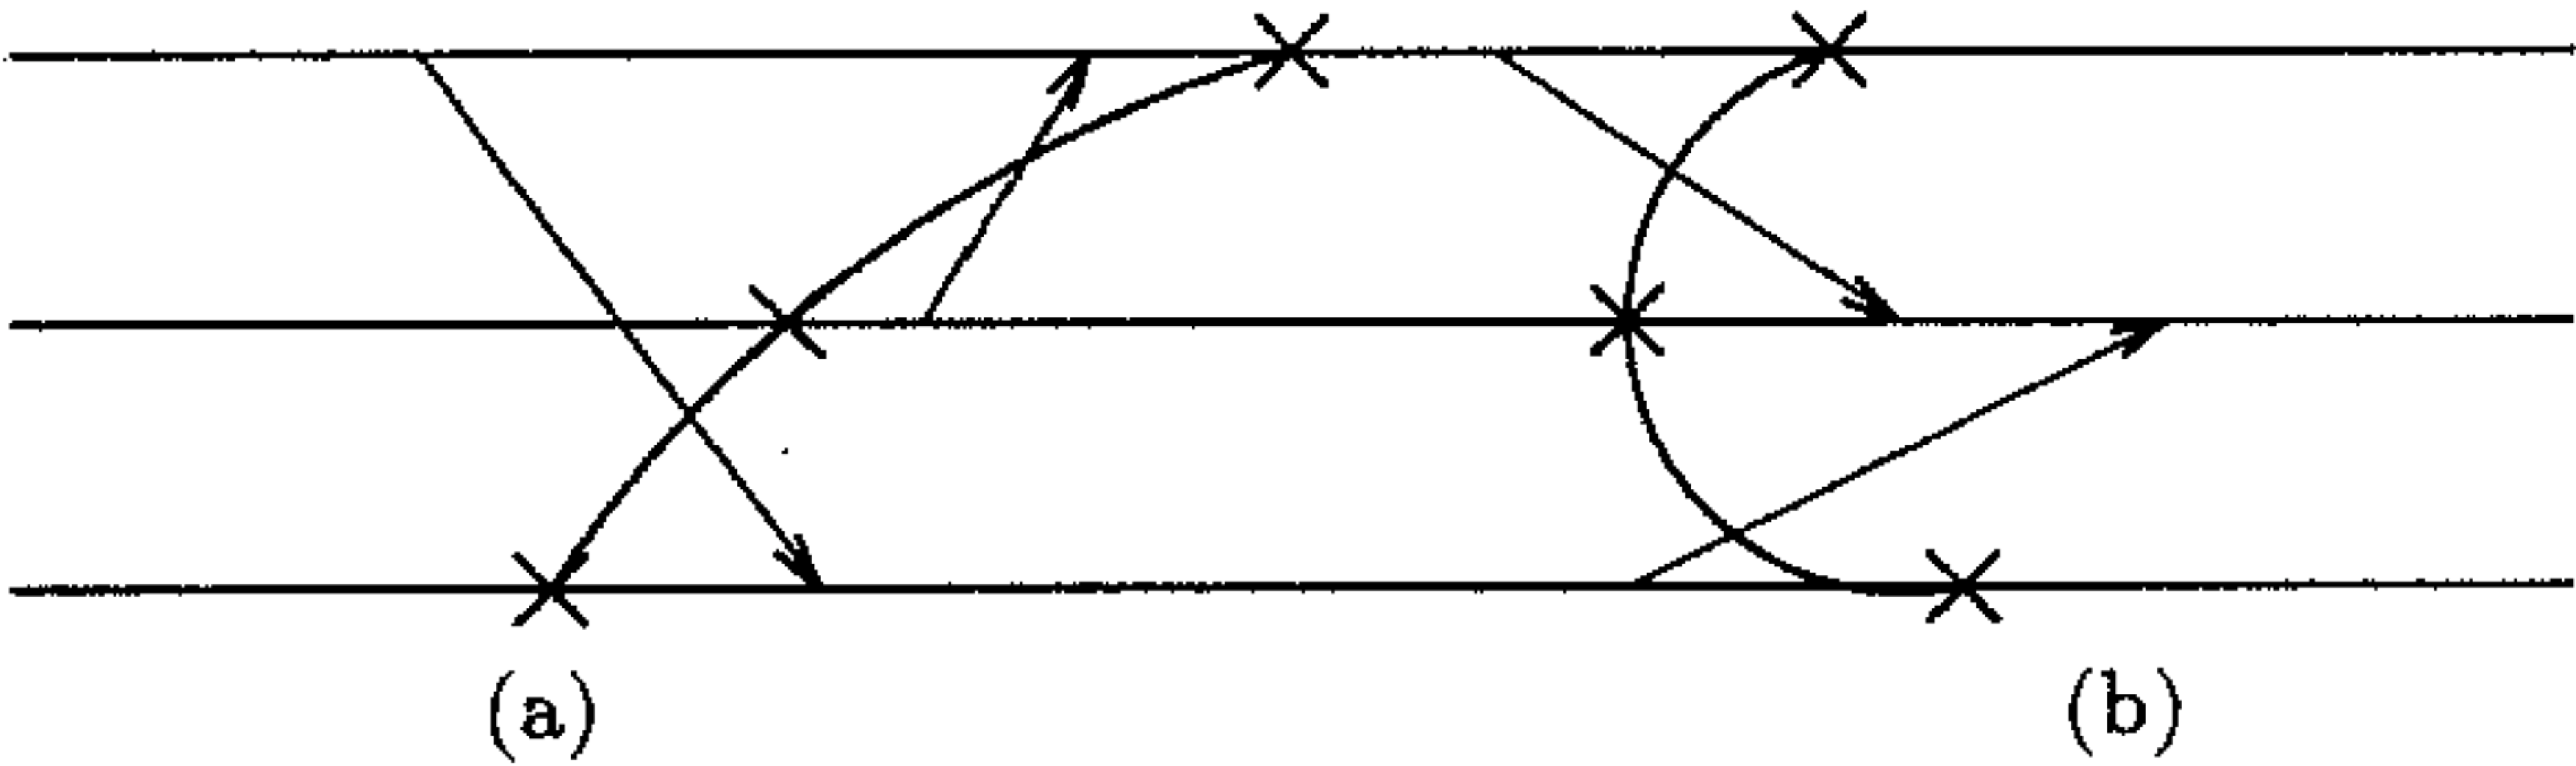
\includegraphics[width=0.8\textwidth]{def_async_sys.pdf}
%  \caption{ \cite{Panangaden1992} }
%\label{pic:fismahistorical}
%\end{figure}
Nachfolgend wird in diesem Kapitel beispielhaft erläutert, wie die Problematik des \textit{cheating husbands}-Rätsel für die Fälle der asynchronen und synchronen Übertragung behandelt werden.

%########################################################################################
% Section: Wissen in asynchronen Systemen
%########################################################################################
\subsection{Wissen in asynchronen Systemen}
\label{wissen_sync}
Für die asynchronen Systeme gibt es einen Zusatz in dem Rätsel der \textit{cheating husbands} (\cite{moses1986cheating} et al.). Es beginnt damit, dass Henrietta I verstirbt und damit ihre Tochter (Henrietta II) die Herrschaft von Mamajorca übernimmt. Der letzte Wunsch ihrer Mutter war es, dass Benachrichtungssystem für betrogene Ehefrauen fort zu führen. \\\\
Die Tochter kam der bitte ihrer Mutter nach. Jedoch vollführte sie eine Verbesserung des Systems. Um die Kommunikation zu erleichtern lies Henrietta II Briefkästen an jedem Haushalt in der ganzen Stadt anbringen. Nach dem errichten lies die Königin als erstes einen Brief an alle ausliefern in dem die Neuerungen erläutert wurden und die Eigenschaften des neuen Systems veranschaulicht wurden. Die erste Eigenschaft besagt, dass jeder Brief den die Königin verschickt, wird garantiert, zu einem \textit{nicht vorhersagbaren Zeitpunkt}, eine der Frauen erreichen. Somit ist die zweite Eigenschaft ableitbar aus der ersten. Sie besagt lediglich, dass keine Ankündigungen mehr auf dem Marktplatz gemacht werden müssten.\\\\
Der grundsätzliche Gedanke ist der gleiche. D.h. nach Erhalt der Nachricht wird der untreue Ehemann in der folgenden Nacht erschossen. Aufgrund des zeitversetzten Zustellens der Nachricht gibt es Zustände in einem System, welche nicht vorhersagbar sind. Jenes Problem wird nachfolgend in Theorem \ref{theo_async_1} erläutert.
\begin{theorem}[vgl. Theorem 2, \cite{moses1986cheating} S. 168]\\
\label{theo_async_1}
Wenn mehr wie ein untreuer Ehemann existiert und die originalen Anweisungen gelten, so sind diese über einen asynchronen Kanal zu versenden und somit wird kein Ehemann erschossen.
\end{theorem}
\begin{proof}
Der Beweis ist durch Veranschaulichung des Ablaufes leicht zu erbringen. Durch die asynchrone Verteilung der Briefe und die Tatsache das es eine eventuelle Verteilung dieser Briefe gibt handelt es sich um "'eventual common knowledge"' (siehe Kap. \ref{GemeinsamesWissen}). Wird nun ein Brief von der Königin versendet, erhält jede Frau eventuell den Brief, der für sie bestimmt war und die besagt Frau weiß ebenfalls, dass es eventuell noch weitere Frauen gibt, die einen Brief erhalten haben könnten. Es gibt keine Sicherheit für die Frauen um fest zu stellen, ob ihr Ehemann zweifelsfrei einer der untreuen ist. Zweifelsfrei kann sich dies deshalb nicht sagen lassen, da die Frau nicht weiß ob die ruhigen Nächte auf der Tatsache basieren, dass die anderen Briefe noch nicht zugestellt wurden oder ob es eine Reaktion andere Frauen auf den Erhalt eines Briefes ist.$\square$
\end{proof}
Aus dem Beweis resultiert, dass sich die Frauen auf Grund der Unsicherheit nie dazu entschließen würden, ihren Gemahlen zu erschießen, denn es könnte sich ja auch um einen Irrtum handeln, da noch nicht alle Briefe zugestellt wurden.\\\\
Dieses Verhalten lässt sich auf verteilte Wissen übertragen. Mit diesem Ansatz ohne jegliche Verbesserungen, wie bereits vorgestellt, kann in asynchron verteilten Systemen nicht festgestellt werden ob die Nachricht angekommen ist oder nicht. Es operiert nach dem Prinzip "'Fire and Forget"'. Dies bedeutet, die Nachricht wird gesendet und was im Anschluss mit der Nachricht passiert, d.h. ob diese ankommt beim Kommunikationspartner oder verloren geht, spielt für den Sender keine Rolle mehr.$\square$\\\\
Für einen Ansatz mit asynchronen Systemen, in welchem es eine Bestätigung bzw. Quittung auf den Erhalt der Nachricht gibt, befassen sich auch andere Darstellungen. Eine von ihnen ist das Problem der byzantinischen Generäle. Hierbei stimmen sich zwei räumlich getrennte Generäle, durch das aussenden eines Boten, ab um gemeinsam eine im Tal liegende Armee anzugreifen. Dieser Bote muss allerdings durch das Tal, in welchem sich die feindlich gesinnte Armee befindet. Durch diesen Umstand kann diese Nachricht, ebenfalls verloren oder durch eine falsche Nachricht mittels eines Boten von der anzugreifenden Armee ersetzt werden. Gesetzt dem Fall der Bote wird nicht abgefangen, so erhält der Bote eine Quittierung über den Erhalt der Nachricht und wird auf den Rückweg ausgesendet. Der General quittiert wiederum die Nachricht, dass er die Bestätigung seines Kollegen erhalten hat. Hierbei lässt sich leicht ausmachen, dass es schnell in einen endlosen Kreis der Bestätigung Enden kann. Somit ist es in asynchron verteilten Systemen auch nicht allein mit dem Senden von Bestätigungen getan. Diese würden zu viel Belegung der Kanäle nach sich ziehen.


%########################################################################################
% Section: Wissen in synchronen Systemen
%########################################################################################

\subsection{Wissen in synchronen Systemen}
\label{wissen_sync}
Für Wissen in synchronen Systemen wird in zwei Bereiche unterteilt. Zum einen in schwache, zum anderen in starke synchrone Systeme. In beiden Bereichen, wird wieder die Erzählung der "'cheating Husbands"' aufgegriffen und ausgebaut.
\subsubsection{Schwache synchrone Systeme}
\label{schwach_sync_wissen}
Bei schwachen synchronen Systemen wird zunächst gewährleistet, dass jeder Kommunikationsteilnehmer die Nachricht erhält. Wie dieser Mechanismus ausgeführt werden kann, wird im Nachgang aufgezeigt (Vgl. \cite{moses1986cheating} S. 170-171).\\\\
In der Geschichte wird Henrietta II von Henrietta III beerbt. Diese will ebenfalls das Benachrichtigungssystem fortführen. Wie ihre beiden Vorgängerinnen hat auch Henrietta III eine Idee wie das bisherige System verbessert werden könnte. Diese Verbesserung sieht vor, dass jeder Brief innerhalb einer gesetzten Grenze von b Tagen ihr Ziel erreicht. Für das Festlegen einer Grenze b wird von den Autoren der Begriff des „b-common-knowledge“ eingeführt. Es sagt aus, dass innerhalb von b Tagen jede Frau über das gleiche Wissen verfügt.\\\\
Für schwache synchrone Systeme führen die Autoren mehrere Annahmen ein, welche auch bewiesen werden. In dieser Ausarbeitung wird sich mit der Grundannahme auseinandergesetzt. Die weiterführenden Annahmen können in (\cite{moses1986cheating} S. 170-171) nachgeschlagen werden.

\begin{satz} [vgl. Proposition 3, \cite{moses1986cheating} S. 170-171]
\label{prop_weak_sync}
In schwachen synchronen Systemen mit einer Grenze b beim Ausliefern der Briefe, weiß eine Frau exakt von k untreuen Ehemännern, wenn k*b stille Nächte, nach dem Erhalt des Briefes vorüber gegangen sind.
\end{satz}
\begin{proof}\hfill\\
Im Ausgangszustand weiß eine Frau von keinen untreuen Ehemännern (k=0). Nach k*b=0 leisen Nächten kann besagte Ehefrau den Rückschluss führen, dass ihr Ehemann untreu ist. Durch den letzten Brief der aktuellen Königin, weiß die Frau nicht vorher, dass ihr Mann untreu sei. \\Es kann nun angenommen werden, dass eine Frau von k untreuen Ehemännern weiß. Um feststellen zu können, dass ihr eigener Ehemann Untreu ist müssen k*b ruhigen Nächte vorangegangen sein. Wenn eine Frau weiß, das Ihr Mann treu ist, dann weiß jede betrogene Frau von k untreuen Männern, welche durch Induktion nacheinander ihren Mann erschießen, wenn k*b stille Nächte, nach Erhalt des Briefes, vorangegangen sind.\\ Wenn eine Frau weiß, ihr Ehemann ist treu und die erste betrogene Frau einen Brief einen Tag zuvor Erhält (b-1) erhält. So ist es möglich, dass keine Schüsse vor der $(k+1)b^{th}$ Nacht, nach Erhalt des Briefes fallen. So weiß die Frau mit der Annahme ihr Mann wäre treu, dass er dies doch nicht ist.
$\square$
\end{proof}
Es wird in diesem Zusammenhang von einem schwachen synchronen System gesprochen, da es durchaus noch zu Zuständen kommen kann, welche in Unsicherheiten resultieren. \\So ist es denkbar, dass Frauen von lauten Nächten verunsichert werden. Dies ist wie folgt zu erläutern. Es gibt zwei Frauen (nachfolgend als 1 und 2 bezeichnet). 1 weiß, dass der Ehemann von 2 untreu ist. 1 erhält am Montag einen Brief von der Königin. In der Nacht nachdem Frau 1 den Brief erhalten hat, hört diese wie Frau 2 Ihren Ehemann erschießt. Nach diesem Schuss herrscht Unsicherheit bei Frau 1. Diese Unsicherheit wird durch die Zustellzeitpunkte der Briefe hervorgerufen. Hierfür gibt es nun zwei Theorien. Die erste ist, der bereits dargestellte Vorgang, dass Frau 2 Ihren Mann erschießt. Der zweite Fall ist problematischer.\\ Wird nun davon ausgegangen, dass Frau 2 den Brief bereits am Sonntag erhält und weiß, dass der Mann von Frau 1 untreu ist, fällt in der nachfolgenden Nacht kein Schuss und Frau 2 weiß ihr Mann ist untreu. \\
Begründet durch diese Unsicherheiten handelt es sicher hierbei um schwach synchrone Systeme. 

\subsubsection{Starke synchrone Systeme}
\label{stark_sync_wissen}
Für die Erläuterung von starken synchronen Systemen wird die Erzählung wieder erweitert erbt eine neue Königin den Thron. Diese bringt ebenfalls eine eigene Erweiterung des bisherigen Systems mit. Hierbei wird sich mit der Einführung eines Kalenders beholfen.\\\\ 
Mittels eines kalendarischen Systems können exakte Aussagen getroffen werden. Problematisch ist es wenn ein Teilnehmer sich nicht an dieses System hält. So können Ergebnisse verfälscht werden. Im Bezug auf die Erzählung bedeutet dies, wenn eine Frau ungehorsam ist und ihren Mann z.B. nicht erschießt, so erschießen die anderen Frauen fälschlicher Weise Ihre Männer, da diese auf Grund der ruhigen Nacht annehmen Sie wäre untreu.\\\\
In \ref{theo_sync_1} wird nachfolgend ein Beweis geführt, der verdeutlicht, wie folgsame Frauen zu den richtigen Erkenntnissen gelangen durch starke synchrone Systeme. 
\begin{theorem}[vgl. Theorem 2, \cite{moses1986cheating} S. 168]\\
\label{theo_sync_1}
Im Fall von stark synchronen Systemen, wenn es der Fall ist, dass es gemeinsames Wissen ist, dass mindestens eine folgsame Frau existiert, so erschießen alle folgsame Frauen ihre Ehemänner.
\end{theorem}
\begin{proof}
Wenn man annimmt es gäbe nur einen untreuen Ehemann, dann müsste die Ehefrau diesen erschießen. Aufgrund der Annahme, es gäbe eine folgsame Ehefrau, müsste diese ihren Mann erschießen.\\
Sind es exakt zwei betrogene Frauen (k=2) handeln diese nach folgendem Grundsatz: "' Wenn mein Mann treu ist, so muss die betrogene Frau, welche ich kenne die folgsame sein"'. Somit wird der Ehemann entsprechend nach b-1 (bzw. spätestens nach b) Tagen erschossen. Wenn bis dahin keine Schüsse gefallen sind (b+1 Tage), dann weiß die Frau, dass es ihr Ehemann ist, der untreu gewesen ist und erschießt diesen in der Nacht. Gibt es nun k $\geq$ 2 untreue Männer, so werden alle von den folgsamen Frauen nach (b+k-1) Nächten erschossen.\\
Sind es exakt k+1 untreue Männer, kennt jede folgsame Frau exakt k untreue Männer und weiß somit, wenn ihr Ehemann treu ist, wird  nach (b+k-1) Nächten ein untreuer Mann erschossen. Tritt nun der Fall ein, dass die Nacht ruhig blieb und weiß die Ehefrau mit dem vermeintlich treuen Ehemann, dass sie diesen Erschießen muss. Dies geschieht nach (b+(k+1)-1) Nächten. \\ Der Beweis kann mittels Induktionsverfahren nachvollzogen werden.
$\square$
\end{proof}
So lässt sich über stark synchrone Systeme sagen, wenn alle Prozesse oder Teilnehmer folgsam gegenüber den Rahmenbedingungen sind, werden Sie alle über ein gemeinsames Wissen verfügen, welches nahezu fehlerfrei läuft.
\section{Varianten des gemeinsamen Wissens}
\label{GemeinsamesWissen}
In Kap. 4 wurden bereits asynchrone Systeme dargestellt. Dieses Kapitel behandelt Erweiterungen für asynchrone Systeme um einen Grad an Zuverlässigkeit zu gewährleisten. Die Prozesse müssen Vereinbarungen treffen. Dies bedeutet, dass es eine Simultanität unter den Prozessen geben wird. 
%########################################################################################
% Section: Epsilon common knowledge
%########################################################################################
\subsection{Epsilon common knowledge}
\label{epsilon_comm_know}
Eine Art der Vereinheitlichung in asynchronen Systemen kann mit Hilfe von Zeiteinheiten gewährleistet werden. Sie werden als Epsilon Zeiteinheiten bezeichnet. Da es keine genauen Zeiteinheiten in asynchronen Systemen gibt, wird mit diesen Zeiteinheiten gearbeitet. Jeder Prozess verfügt innerhalb dieser Zeiteinheiten über ein gemeinsames Wissen.\\\\ Sie sind wie nachfolgend definiert:
\begin{itemize}
			\item $E^\epsilon$, jeder Prozess erhält innerhalb von $\epsilon$ Zeiteinheiten die Nachricht
			\item $C^\epsilon(\phi) $, größter Fixpunkt von X
			\item $X=E^\epsilon(\phi \wedge X) $, X ist die freie Variable im Fixpunkt-Operator 
			%\widehat{=} => entspricht-Zeichen
		\end{itemize}
Der größte Fixpunkt für das gemeinsame Wissen wird in C sichtbar.
%########################################################################################
% Section: Wissen in asynchronen Systemen
%########################################################################################
\subsection{Eventual common knowledge}
\label{eventual_comm_know}
Bei eventuellem gemeinsamen Wissen treffen die Prozesse Vereinbarungen in einem globalen Status der Ausführung. Sie kann konsistent sein, muss dies aber nicht sein. Hieraus wird grundsätzlich eine Basis für gemeinsames Wissen geschaffen. \\\\
Eventuelles gemeinsames Wissen wird wie folgt definiert:
\begin{itemize}
			\item $E^\Diamond$, jeder Prozess hat eventuell das Wissen (zu einem Zeipunkt der Ausführung)
			\item $C^\Diamond(\phi) $, größter Fixpunkt von X
			\item $X=E^\Diamond(\phi \wedge X) $

\end{itemize}

%########################################################################################
% Section: Wissen in asynchronen Systemen
%########################################################################################
\subsection{Timestamped common knowledge}
\label{timestamped_comm_know}
Bei gemeinsamem Wissen basierend auf Zeit wird mit Hilfe der lokalen Zeit der einzelnen Prozesse gearbeitet. Sie basiert darauf, dass die einzelnen Prozesse einen lokalen Status erreichen, in dem sie die gleiche lokale Zeit besitzen. Im theoretischen Fall, dass alle asynchronen Prozesse die gleiche lokale Zeit hätten, wäre es ein reguläres gemeinsames System. D.h. kein asynchrones System. \\\\
Die Definition sieht wie folgt aus:
\begin{itemize}
			\item $K^T_i(\phi)$, Prozess \textit{i} weiß $\phi$ zum lokalen Zeitpunk T
			\item $E^T(\phi) = \bigwedge_i K^T_i(\phi) $ und $C^T(\phi)$, größter Fixpunkt von X
			\item $X=E^T(\phi \wedge X)$

		\end{itemize}
%########################################################################################
% Section: Wissen in asynchronen Systemen
%########################################################################################
\subsection{Concurrent common knowledge}
\label{concurrent_comm_know}
Bei gleichzeitigem gemeinsamen Wissen wird mit Schnittpunkten gearbeitet. Wenn die Prozesse gemeinsames Wissen austauschen wollen, müssen diese zunächst einen lokalen konsistenten Status einnehmen. \\\\
Im Nachgang folgen die Definitionen für gleichzeitiges gemeinsames Wissen:
	\begin{itemize}
			\item (a,c)	$\models$ $\phi$, wenn Schnittpunk c von Ausführung a = TRUE
			\item (a,c)	$\models$ $K_i(\phi)$, wenn $\forall(a',c')$, $((a',c') \sim_i (a,c) \implies (a',c') \models \phi)$
			\item (a,c)	$\models$ $P_i(\phi)$, wenn $\exists(a,c')$, $((a,c') \sim_i (a,c) \wedge (a,c') \models \phi)$
			\item (a,c)	$\models$ $E^{C^0}(\phi)$, wenn $(a,c) \models \phi$
			\item (a,c)	$\models$ $E^{C^1}(\phi)$, wenn $(a,c) \models \bigwedge_{i\epsilon N}\; K_i P_i(\phi)$
			\item (a,c)	$\models$ $E^{C^k+1}(\phi)$, wenn $(a,c) \models \bigwedge_{i\epsilon N}\; K_i P_i(E^{C^k}(\phi))$ für $k \geq 1$
			\item (a,c)	$\models$ $C^C(\phi)$, wenn $(a,c) \models X = E^C(X \wedge \phi)$ 
			$C^c \implies \bigwedge_{k\epsilon Z*}(E^c)^k(\phi) $ 
		\end{itemize}
Im Operator E weiß jeder Prozess im gegebenen Schnitt, dass p wahr ist in irgendeinem Schnitt, welcher mit dem eigenen lokalen Schnitt p konsistent ist. \\\\ 
Durch den Operator C wird ein konsistenter Schnitt erreicht. D.h. in einem konsistenten Zustand mit eigenem lokalen Schnitt wird p wahr und alle anderen Prozesse haben das gleiche gemeinsame Wissen. Es bleibt noch anzumerken, dass die Prozesse allen Protokollen unterliegen, welche Vereinbarungen über die Eigenschaften des globalen Status inne haben. \\\\
Um dies etwas praktischer zu Erläutern ist im Nachgang ein Algorithmus abgebildet, mit welchem ein Informationsaustausch bewerkstelligt werden kann: 

\subsubsection{Drei-Phasen Algorithmus}
\begin{figure}[H]
\centering
      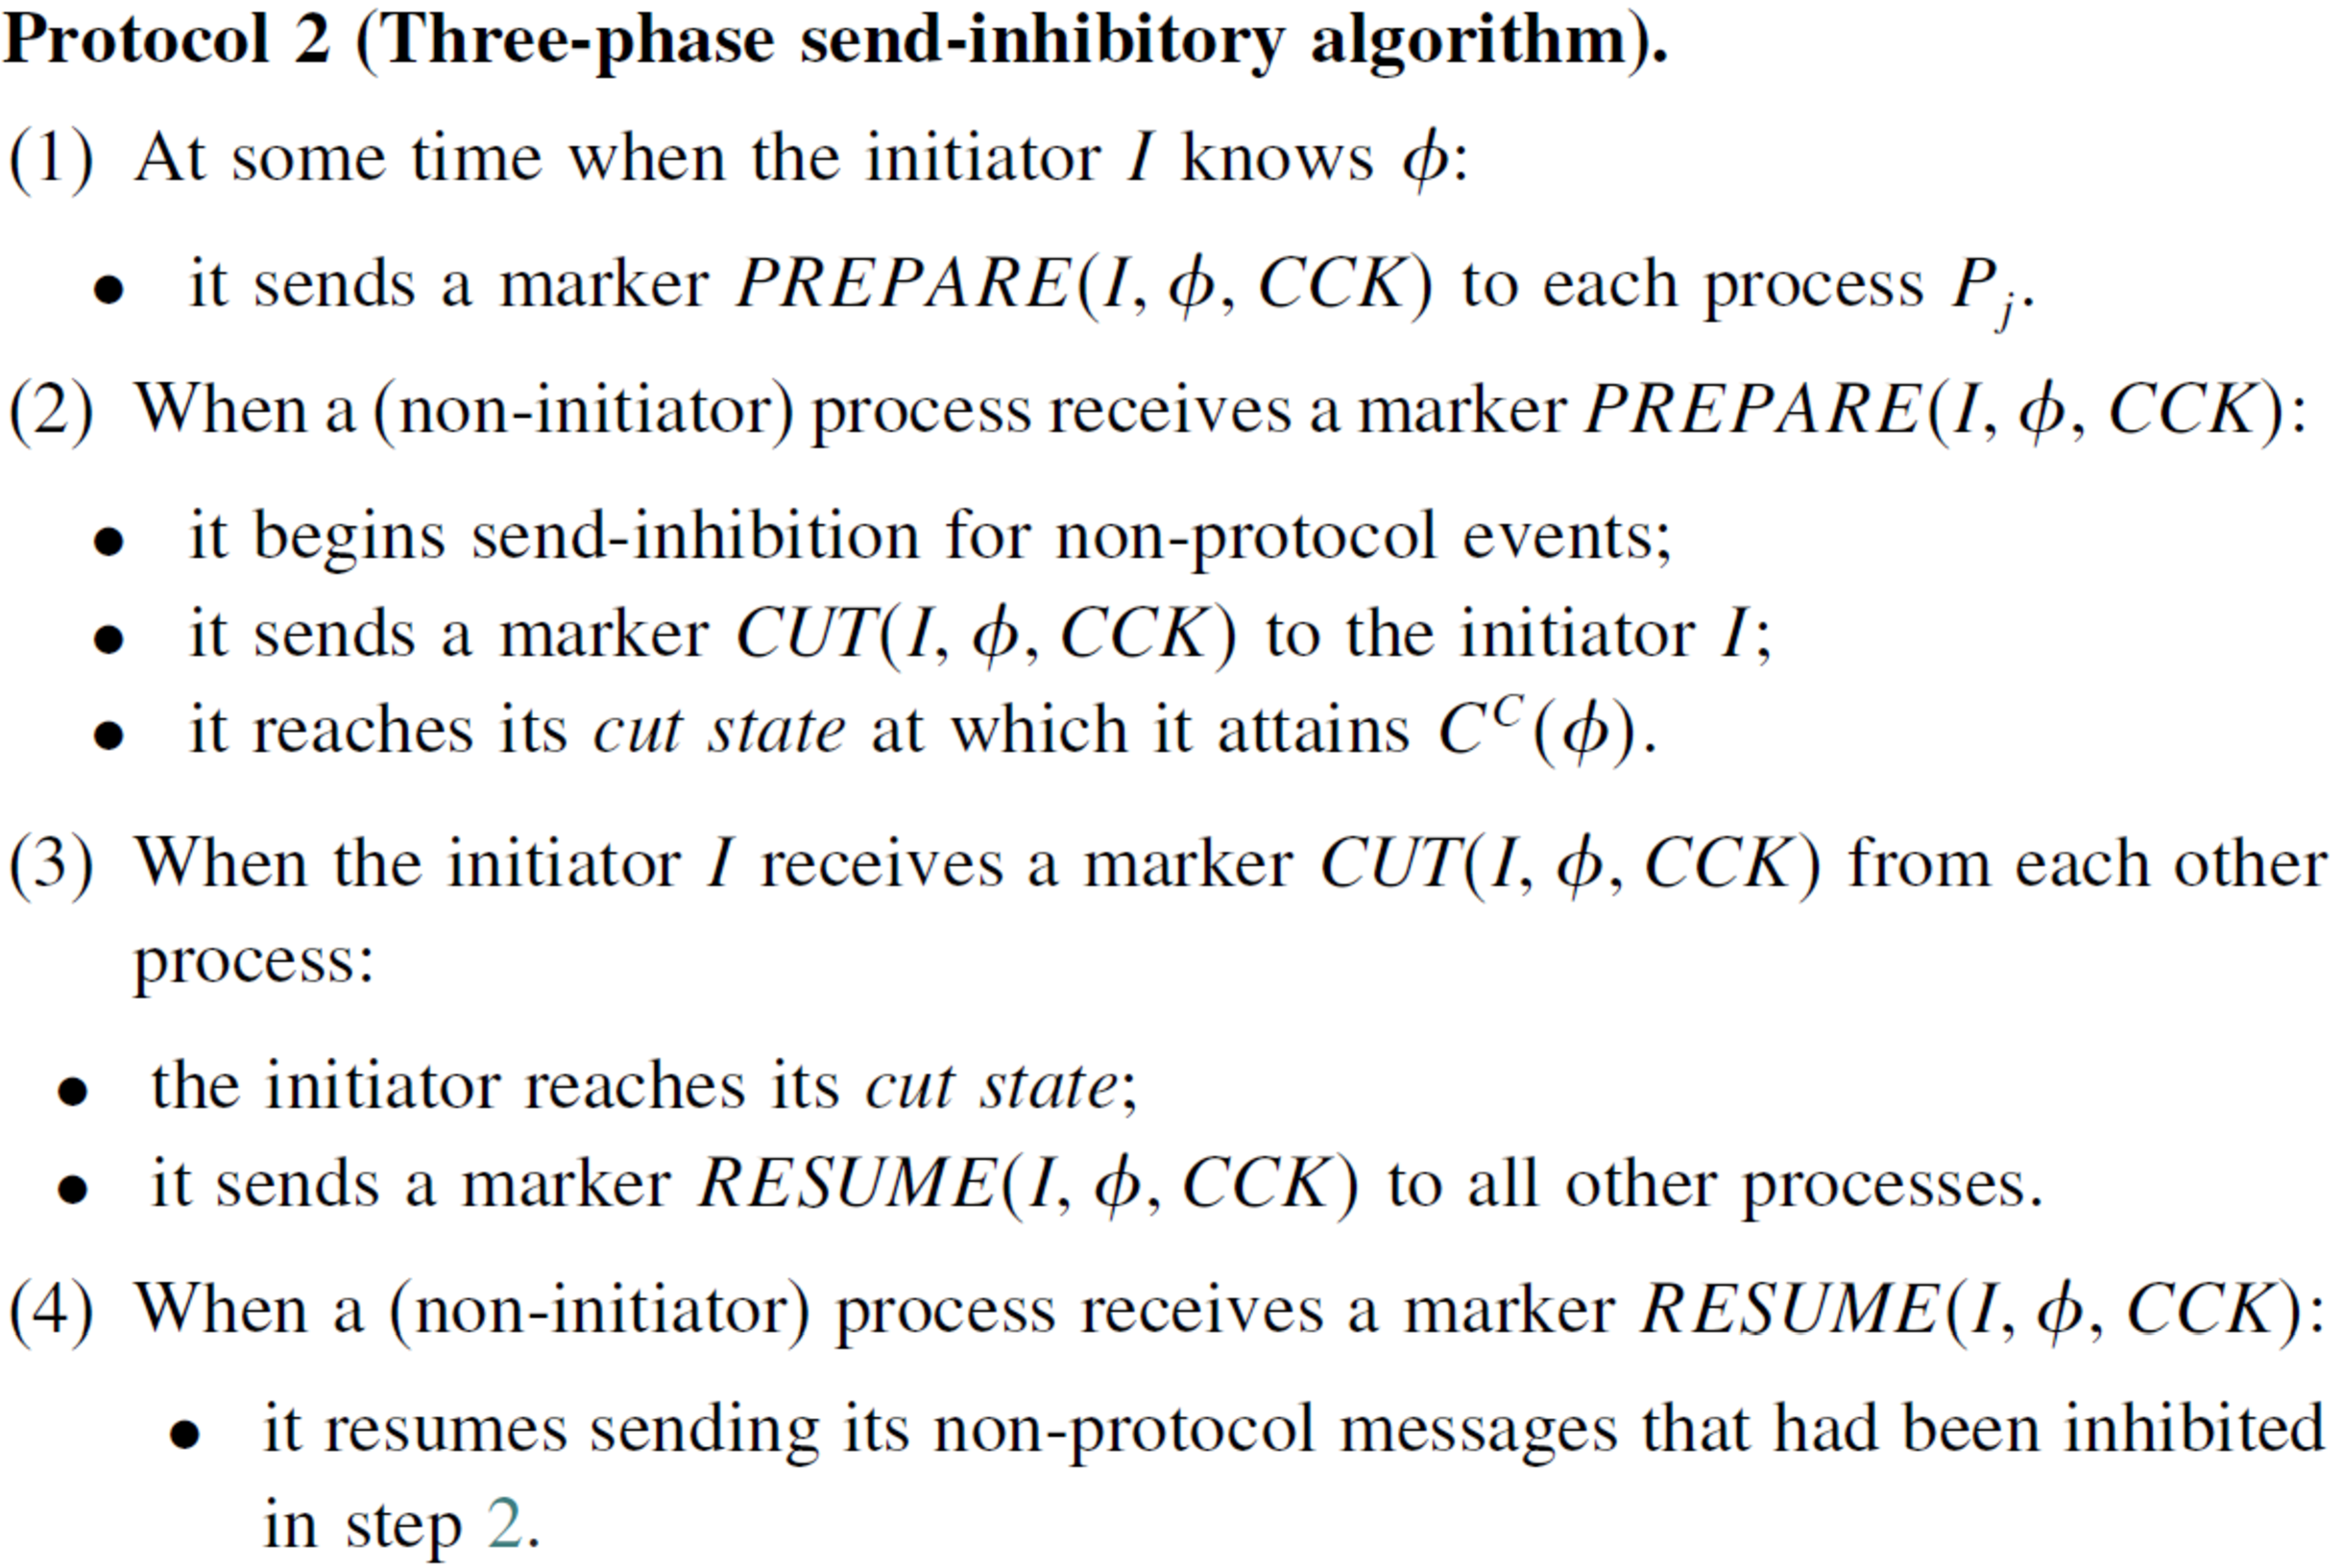
\includegraphics[width=1\textwidth]{three_phase_algo.pdf}
  \caption{ Drei-Phasen Algorithmus für die Gewährleistung von gleichzeitig gemeinsamen Wissen \cite{kshemkalyani2011distributed}}
\label{pic:lbsn}
\end{figure}
Durch den sogenannten Drei-Phasen Algorithmus (Abb. 4) wird gewährleistet, dass alle Prozesse einen Zustand erreichen, welcher einen sicheren und konsistenten Informationsaustausch dient. Er wird in 4 Schritte untergliedert:
\begin{enumerate}
\item Im ersten Schritt sendet ein Initiator eine Nachricht aus, um die anderen Prozesse auf einen Informationsaustausch vorzubereiten.
\item Nachdem der Prozess diese Nachricht erhalten hat, werden zunächst alle anderen Operationen gesperrt und ein konsistenter Zustand eingenommen, ehe der Initiator benachrichtigt wird, dass der Prozess bereit für einen Informationsaustausch ist.
\item Nachdem der Initiator von allen Prozessen benachrichtigt wurde, dass diese bereit für den Austausch sind, erreicht dieser selbst einen konsistenten Zustand und benachrichtigt die anderen.
\item Im letzten Schritt findet nun der eigentliche Nachrichtenaustausch statt. 
\end{enumerate}

Der Algorithmus ist sehr klar strukturiert und bietet die Möglichkeit von sicherer Übertragung von Informationen. So kann innerhalb von asynchronen Systemen mit Daten gearbeitet werden, welche auf gemeinsamen Wissen beruhen ohne das es Unsicherheiten im Bezug auf die Teilnehmer gibt. 
\section{Zusätzliche Kommunikation}
\label{Kommuniaktion}
In den bisherigen Betrachtungen der Varianten zum \textit{cheating-husbands}-Rätsel war die Kommunikationsfähigkeit zwischen den Ehefrauen stark eingeschränkt.
Die Kommunikation einer Ehefrau war darauf beschränkt mitzuteilen, ob sie weiß, dass sie betrogen wurde. 
Wenn sie dies mit Sicherheit sagen konnte, erschießt sie ihren Ehemann in der Nacht, die anderen Ehefrauen hörten den Schuss und wussten somit, dass eine andere Ehefrau sich sicher war, dass ihr Ehemann betrogen hat.\\
Wenn diese Beschränkung etwas gelockert wird, können ohne die Mächtigkeit des Systems signifikant zu erhöhen, wesentlich effizientere Kommunikationsprotokolle genutzt werden, um das Problem zu lösen.
Um dies zu zeigen abstrahieren wir nun wieder von dem, als sehr entscheidend festgestellten, Nachrichtensystem. 
Nachrichten der Königin werden daher ohne Verzögerung verteilt, und jeder Ehefrau ist dies bekannt.
Bei der ursprünglichen Lösung aus der Motivation wurde das Problem in n Tagen Tagen korrekt gelöst, wobei n die Anzahl der untreuen Ehemänner ist.
Y. Moses et al. \cite{moses1986cheating} (vgl. S.175) zeigen, dass das Problem mit zusätzlicher Kommunikation mit einem Algorithmus gelöst werden kann, der höchstens drei Tage benötigt. Dabei wird die Kommunikationsfähigkeit der Ehefrauen um das Schießen in die Luft ergänzt. Eine \glqq Nachricht\grqq{} einer Ehefrau ist somit nicht mehr an ihr Wissen über die Untreue ihres Ehemannes gekoppelt.
Die Mächtigkeit des Systems wird dabei insofern auf ähnlichem Niveau gehalten, als das weiterhin nur über Schüsse um Mitternacht kommuniziert werden kann. Dies entspricht einer binären Nachricht pro Nacht, ein oder mehrere Schüsse sind in der Nacht gefallen oder keiner.\medskip

Das \textit{cheating husbands}-Rätsel mit dieser Erweiterung der erlaubten Kommunikation kann auch technischer formuliert werden (vgl. \cite{moses1986cheating} S. 175): 
In einem verteilten System soll das Konsens-Problem gelöst werden. Die Prozesse haben einen gemeinsamen Speicher von einem Bit. Es gibt maximal zwei verschiedene Werte im System, diese unterscheiden sich nur um eins.\\
Die Analogie zum \textit{cheating husbands}-Rätsel kann gezogen werden, denn auch dort wird das Konsens-Problem gelöst, da sich alle Ehefrauen auf die korrekte Anzahl untreuer Ehemänner einigen muss.
Es gibt zwei unterschiedliche Annahmen von der korrekten Anzahl untreuer Ehemänner und die entsprechenden Zahlen unterscheiden sich nur um eins. Die betrogenen Ehefrauen kennen einen untreuen Ehemann weniger, als die nicht betrogenen.
Durch die Erweiterung der Kommunikation um das in die Luft Schießen kann das Schießen als die freie Belegung eines gemeinsamen Speichers auf den Wert 1 angesehen werden, fällt kein Schuss wird der Wert auf 0 gesetzt.
Der Wert des gemeinsamen Speichers ist jeder Ehefrau bewusst.
\medskip

Zunächst können wir nun mit einer an \cite{moses1986cheating} angelegten Überlegung beweisen, dass es kein Protokoll gibt, das weniger als drei Nächte unabhängig von der Probleminstanz benötigt:\\

Betrachten wir eine Probleminstanz mit k untreuen Ehemännern.
Im Allgemeinen kann es nun zwei verschiedene Anzahlen von untreuen Ehemännern geben, von denen die Ehefrauen wissen.
Entweder kennen sie alle k, wenn sie selbst nicht betrogen wurden, oder sie kennen $k-1$, wenn sie betrogen wurden.
Die Anzahl untreuer Ehemänner, von denen die i-te Ehefrau weiß, werde nun als $k_i$ bezeichnet.
Da keine der Ehefrauen weiß, ob sie selbst betrogen wurden, weiß jede von ihnen nur, dass die wahre Anzahl untreuer Ehemänner entweder $k_i$ oder $k_i+1$ ist.
Somit gibt es Ehefrauen die wissen, dass es $k-1$ oder $k$ und welche die wissen, dass es $k$ oder $k+1$ untreue Ehemänner gibt.
Insgesamt gibt es also drei verschiedene Anzahlen untreuer Ehemänner aus denen die richtige Anzahl bestimmt werden muss.
Wenn die wahre Anzahl untreuer Ehemänner bekannt ist, ist das System vollständig bestimmt, jede Ehefrau weiß dann, ob sie ihren Mann erschießen muss.
Jede Nacht kann allerdings nur eine binäre Information bekannt gemacht werden, daher kann im Allgemeinen jede Nacht nur einer der drei möglichen Anzahlen von untreuen Ehemännern ausgeschlossen werden.

So könnte ein Schuss in der ersten Nacht bedeuten, dass es entweder $k-1$ oder $k$ untreue Ehemänner sind.
Eine zweite Nacht müsste dann noch abgewartet werden, um eindeutig zu bestimmen, welcher der beiden Fälle der Wahrheit entspricht.
Beispielsweise würde ein weiterer Schuss in der zweiten Nacht bedeuten, dass es tatsächlich $k-1$ untreue Ehemänner sind.
Wenn kein Schuss in der ersten Nacht fallen würde, wäre bereits klar, dass es weder $k-1$ noch $k$ untreue Ehemänner sind, sodass es $k+1$ sein müssen. Es kann also durchaus Fälle geben, in denen das Problem in zwei Nächten gelöst ist. Es kann aber kein Protokoll geben, dass das Problem unabhängig von $k$ immer in weniger als drei Nächten löst.\\

\subsection{Protokoll mit zusätzlicher Kommunikation}

Die folgende leicht modifizierte Version des Kommunikationsprotokolls von Y. Moses et al. \cite{moses1986cheating} (vgl. S.175) ist eine optimale Lösung für das \textit{cheating husbands}-Rätsel mit zusätzlicher Kommunikation, in dem Sinne, dass es maximal drei Tage benötigt, um jegliche Probleminstanz korrekt zu lösen:

\begin{itemize}
	\item 1. Falls eine Ehefrau von $k_1$ (mit $k_1 \text{ mod } 3 = 1$) untreuen Ehemännern weiß, schießt sie in der ersten Nacht in die Luft.
	\item 2. Falls eine Ehefrau von $k_2$ (mit $k_2 \text{ mod } 3 = 2$) untreuen Ehemännern weiß und in der ersten Nacht kein Schuss gefallen ist, erschießt sie ihren Ehemann in der zweiten Nacht.
	\item 3. Falls eine Ehefrau von $k_0$ (mit $k_0 \text{ mod } 3 = 0$) untreuen Ehemännern weiß und in der ersten Nacht ein Schuss gefallen ist, erschießt sie ihren Ehemann in der zweiten Nacht.
	\item 4. Falls in den ersten beiden Nächten kein Schuss gefallen ist und $k_0 \ne0$, erschießen alle Ehefrauen ihren Mann in der dritten Nacht.
	\item 5. Falls in der ersten Nacht ein Schuss gefallen ist, in der zweiten Nach kein Schuss zu hören war, erschießen alle Ehefrauen, die in der ersten Nacht bereits geschossen haben, ihren Mann in der dritten Nacht. 
\end{itemize}
Das Protokoll kann folgendermaßen erklärt werden:\\
(Zu 1.) In der ersten Nacht wird die Fallunterscheidung gemacht, ob es Ehefrauen gibt, die von $k_1$ untreuen Ehemännern wissen oder nicht.
(Zu 2.) Falls in der ersten Nacht nicht geschossen wurde, ist bereits bekannt, dass es höchstens Ehefrauen geben kann, die von $k_0$ oder $k_2$ untreuen Ehemännern wissen. Alle Ehefrauen, die von $k_2$ untreuen Ehemännern wissen, können ihren Mann nun töten, denn entweder wissen alle Ehefrauen von $k_2$ untreuen Ehemännern, dann sind alle betrogen wurden, oder die Ehefrauen, die nur $k_2$ untreue Ehemänner kennen, wissen von einem weniger, als die, die $k_0$ kennen.
(Zu 3.) Falls in der ersten Nacht geschossen wurde, können die Frauen, die von $k_0$ untreuen Ehemännern ihren Ehemann erschießen. Die Begründung verläuft analog zu der vorherigen, da es nun nur Ehefrauen geben kann, die von $k_0$ oder $k_1$ untreuen Ehemännern wissen.
(Zu 4.) Falls in den ersten beiden Nächten kein Schuss gefallen ist, wissen alle Ehefrauen von $k_0$ untreuen Ehemännern, sodass es entweder keinen einzigen untreuen Ehemann gibt, dann passiert nichts, oder alle Ehemänner waren untreu, dann werden alle erschossen.
(Zu 5.) Falls in der ersten Nacht Schüsse fielen in der zweiten jedoch nicht, kann es nur Ehefrauen geben, die von $k_1$ oder $k_2$ untreuen Ehemännern wissen. Aus einem analogen Argument, wie zu 1. und 2. können dann die Ehefrauen, die von $k_1$ untreuen Ehemännern wissen, ihren Ehemann erschießen.\medskip

Die Fähigkeit untereinander zu Kommunizieren ermöglicht es, dass in diesem Kommunikationsprotokoll keine Notwendigkeit darin besteht, dass die Königin verkündet, dass es mindestens einen untreuen Ehemann gibt. Tatsächlich funktioniert das Protokoll auch für den Fall, dass es keinen einzigen untreuen Ehemann gibt.
Mit Hilfe der Veranschaulichung von Kripke-Modellen können wir nun die korrekte Funktionsweise des Protokolls an dem Beispiel aus Kapitel \ref{Kripke-Modelle} betrachten, bei dem (0,1,1) der wahre Zustand war:\\
Von der ersten zur zweiten Nacht wird der in Abbildung \ref{kom_(0,1,1)_1} dargestellte Übergang vollzogen, das Problem wird also direkt gelöst.
Die tatsächliche Anzahl der untreuen Ehemänner im Zustand (0,1,1) ist $k=2$. Die Ehefrauen 2 und 3 kennen $k_1 = 1$ untreue Ehemänner und Ehefrau 1 weiß von allen $k_2 = 2$ untreuen Ehemännern.
In der ersten Nacht schießen die beiden Ehefrauen mit $k_1$ in die Luft. Es gibt also mindestens einen untreuen Ehemann und höchstens zwei.
Dementsprechend sind in Abbildung \ref{kom_(0,1,1)_1} die Zustände (0,0,0) und (1,1,1) ausgeschlossen worden.

\begin{figure}
	\begin{tikzpicture}[thick,scale=0.2]
	\coordinate[label={180:\text{(1,0,0)}}] (UVL) at (0,0,12);
	\coordinate[label={0:\text{(1,1,0)}}] (UVR) at (12,0,12);
	\coordinate[label={180:\text{(0,0,0)}}] (OVL) at (0,12,12);
	\coordinate[label={-120:\text{(0,1,0)}}] (OVR) at (12,12,12);
	\coordinate[label={-86:\text{(1,0,1)}}] (UHL) at (0,0,0);
	\coordinate[label={0:\text{(1,1,1)}}] (UHR) at (12,0,0);
	\coordinate[label={180:\text{(0,0,1)}}] (OHL) at (0,12,0);
	\coordinate[label={0:\text{(0,1,1)}}] (OHR) at (12,12,0);
	
	\draw[fill=black] (UVL) circle (8pt);
	\draw[fill=black] (UVR) circle (8pt);
	\draw[fill=black] (OVL) circle (8pt);
	\draw[fill=black] (OVR) circle (8pt);
	\draw[fill=black] (UHL) circle (8pt);
	\draw[fill=black] (UHR) circle (8pt);
	\draw[fill=black] (OHL) circle (8pt);
	\filldraw[color=red] (OHR) circle (8pt);
	
	\draw (UVL) -- node[above] {2} (UVR);
	\draw (UVL) -- node[above left] {1} (OVL);
	\draw (UVL) -- node[left] {3} (UHL);
	\draw (OVR) -- node[above right] {2} (OVL);
	\draw (OVR) -- node[left] {3} (OHR);
	\draw (OVR) -- node[above left] {1} (UVR);
	\draw (OHL) -- node[left] {3} (OVL);
	\draw (OHL) -- node[above] {2} (OHR);
	\draw (OHL) -- node[left] {1} (UHL);
	\draw (UHR) -- node[left] {3} (UVR);
	\draw (UHR) -- node[left] {1} (OHR);
	\draw (UHR) -- node[above left] {2} (UHL);	
	
	\draw[line width=1.5pt,->] (22,8,12) -- node[above] {1. Nacht} (26,8,12); 	
	\end{tikzpicture}
	\qquad
	\hspace*{-0.7cm}
	\begin{tikzpicture}[thick,scale=0.2]
	\coordinate[label={180:\text{(1,0,0)}}] (UVL) at (0,0,12);
	\coordinate[label={0:\text{(1,1,0)}}] (UVR) at (12,0,12);
	\coordinate[label={180:\text{(0,0,0)}}] (OVL) at (0,12,12);
	\coordinate[label={-120:\text{(0,1,0)}}] (OVR) at (12,12,12);
	\coordinate[label={-86:\text{(1,0,1)}}] (UHL) at (0,0,0);
	\coordinate[label={0:\text{(1,1,1)}}] (UHR) at (12,0,0);
	\coordinate[label={180:\text{(0,0,1)}}] (OHL) at (0,12,0);
	\coordinate[label={0:\text{(0,1,1)}}] (OHR) at (12,12,0);
	
	\draw[fill=black] (UVL) circle (8pt);
	\draw[fill=black] (UVR) circle (8pt);
	\draw[fill=black] (OVL) circle (8pt);
	\draw[fill=black] (OVR) circle (8pt);
	\draw[fill=black] (UHL) circle (8pt);
	\draw[fill=black] (UHR) circle (8pt);
	\draw[fill=black] (OHL) circle (8pt);
	\filldraw[color=red] (OHR) circle (8pt);	
	
	\draw (UVL) -- node[above] {2} (UVR);
	\draw (UVL) -- node[left] {3} (UHL);
	\draw (OVR) -- node[left] {3} (OHR);
	\draw (OVR) -- node[above left] {1} (UVR);
	\draw (OHL) -- node[above] {2} (OHR);
	\draw (OHL) -- node[left] {1} (UHL);	
	\end{tikzpicture}
	\caption{Übergang vom ersten zum zweiten Tag im \textit{cheating husbands}-Rätsels mit zusätzlicher Kommunikation ausgehend vom Zustand (0,1,1).}
	\label{kom_(0,1,1)_1}
\end{figure}

Da es keine Ehefrau gibt, die von $k_0$ untreuen Ehemännern weiß, fällt in der zweiten Nacht kein Schuss.
Somit können auch alle Zustände ausgeschlossen werden, in denen es nur einen untreuen Ehemann gibt, sodass das Problem, wie in Abbildung \ref{kom_(0,1,1)_2} zu sehen, nach drei Nächten gelöst ist.

\begin{figure}
	\begin{tikzpicture}[thick,scale=0.2]
	\coordinate[label={180:\text{(1,0,0)}}] (UVL) at (0,0,12);
	\coordinate[label={0:\text{(1,1,0)}}] (UVR) at (12,0,12);
	\coordinate[label={180:\text{(0,0,0)}}] (OVL) at (0,12,12);
	\coordinate[label={-120:\text{(0,1,0)}}] (OVR) at (12,12,12);
	\coordinate[label={-86:\text{(1,0,1)}}] (UHL) at (0,0,0);
	\coordinate[label={0:\text{(1,1,1)}}] (UHR) at (12,0,0);
	\coordinate[label={180:\text{(0,0,1)}}] (OHL) at (0,12,0);
	\coordinate[label={0:\text{(0,1,1)}}] (OHR) at (12,12,0);
	
	\draw[fill=black] (UVL) circle (8pt);
	\draw[fill=black] (UVR) circle (8pt);
	\draw[fill=black] (OVL) circle (8pt);
	\draw[fill=black] (OVR) circle (8pt);
	\draw[fill=black] (UHL) circle (8pt);
	\draw[fill=black] (UHR) circle (8pt);
	\draw[fill=black] (OHL) circle (8pt);
	\filldraw[color=red] (OHR) circle (8pt);
	
	\draw (UVL) -- node[above] {2} (UVR);
	\draw (UVL) -- node[left] {3} (UHL);
	\draw (OVR) -- node[left] {3} (OHR);
	\draw (OVR) -- node[above left] {1} (UVR);
	\draw (OHL) -- node[above] {2} (OHR);
	\draw (OHL) -- node[left] {1} (UHL);	
	
	\draw[line width=1.5pt,->] (22,8,12) -- node[above] {2. Nacht} (26,8,12); 	
	\end{tikzpicture}
	\qquad
	\hspace*{-0.7cm}
	\begin{tikzpicture}[thick,scale=0.2]
	\coordinate[label={180:\text{(1,0,0)}}] (UVL) at (0,0,12);
	\coordinate[label={0:\text{(1,1,0)}}] (UVR) at (12,0,12);
	\coordinate[label={180:\text{(0,0,0)}}] (OVL) at (0,12,12);
	\coordinate[label={-120:\text{(0,1,0)}}] (OVR) at (12,12,12);
	\coordinate[label={-86:\text{(1,0,1)}}] (UHL) at (0,0,0);
	\coordinate[label={0:\text{(1,1,1)}}] (UHR) at (12,0,0);
	\coordinate[label={180:\text{(0,0,1)}}] (OHL) at (0,12,0);
	\coordinate[label={0:\text{(0,1,1)}}] (OHR) at (12,12,0);
	
	\draw[fill=black] (UVL) circle (8pt);
	\draw[fill=black] (UVR) circle (8pt);
	\draw[fill=black] (OVL) circle (8pt);
	\draw[fill=black] (OVR) circle (8pt);
	\draw[fill=black] (UHL) circle (8pt);
	\draw[fill=black] (UHR) circle (8pt);
	\draw[fill=black] (OHL) circle (8pt);
	\filldraw[color=red] (OHR) circle (8pt);		
	\end{tikzpicture}
	\caption{Übergang vom zweiten zum ersten Tag im \textit{cheating husbands}-Rätsels mit zusätzlicher Kommunikation ausgehend vom Zustand (0,1,1).}
	\label{kom_(0,1,1)_2}
\end{figure}

Betrachten wir abschließend noch, veranschaulicht mit Kripke-Modellen, den Spezialfall, dass (0,0,0) der wahre Zustand ist. Alle Ehefrauen kennen also $k_0 = 0$ untreue Ehemänner.
In der ersten Nacht sind keine Schüsse zu hören, sodass alle Zustände mit einem untreuen Ehemann ausgeschlossen werden können. Es ergibt sich die Situation aus \ref{kom_(0,0,0)_1}.

\begin{figure}
	\begin{tikzpicture}[thick,scale=0.2]
	\coordinate[label={180:\text{(1,0,0)}}] (UVL) at (0,0,12);
	\coordinate[label={0:\text{(1,1,0)}}] (UVR) at (12,0,12);
	\coordinate[label={180:\text{(0,0,0)}}] (OVL) at (0,12,12);
	\coordinate[label={-120:\text{(0,1,0)}}] (OVR) at (12,12,12);
	\coordinate[label={-86:\text{(1,0,1)}}] (UHL) at (0,0,0);
	\coordinate[label={0:\text{(1,1,1)}}] (UHR) at (12,0,0);
	\coordinate[label={180:\text{(0,0,1)}}] (OHL) at (0,12,0);
	\coordinate[label={0:\text{(0,1,1)}}] (OHR) at (12,12,0);
	
	\draw[fill=black] (UVL) circle (8pt);
	\draw[fill=black] (UVR) circle (8pt);
	\filldraw[color=red] (OVL) circle (8pt);
	\draw[fill=black] (OVR) circle (8pt);
	\draw[fill=black] (UHL) circle (8pt);
	\draw[fill=black] (UHR) circle (8pt);
	\draw[fill=black] (OHL) circle (8pt);
	\filldraw[color=black] (OHR) circle (8pt);
	
	\draw (UVL) -- node[above] {2} (UVR);
	\draw (UVL) -- node[above left] {1} (OVL);
	\draw (UVL) -- node[left] {3} (UHL);
	\draw (OVR) -- node[above right] {2} (OVL);
	\draw (OVR) -- node[left] {3} (OHR);
	\draw (OVR) -- node[above left] {1} (UVR);
	\draw (OHL) -- node[left] {3} (OVL);
	\draw (OHL) -- node[above] {2} (OHR);
	\draw (OHL) -- node[left] {1} (UHL);
	\draw (UHR) -- node[left] {3} (UVR);
	\draw (UHR) -- node[left] {1} (OHR);
	\draw (UHR) -- node[above left] {2} (UHL);	
	
	\draw[line width=1.5pt,->] (22,8,12) -- node[above] {1. Nacht} (26,8,12); 	
	\end{tikzpicture}
	\qquad
	\hspace*{-0.7cm}
	\begin{tikzpicture}[thick,scale=0.2]
	\coordinate[label={180:\text{(1,0,0)}}] (UVL) at (0,0,12);
	\coordinate[label={0:\text{(1,1,0)}}] (UVR) at (12,0,12);
	\coordinate[label={180:\text{(0,0,0)}}] (OVL) at (0,12,12);
	\coordinate[label={-120:\text{(0,1,0)}}] (OVR) at (12,12,12);
	\coordinate[label={-86:\text{(1,0,1)}}] (UHL) at (0,0,0);
	\coordinate[label={0:\text{(1,1,1)}}] (UHR) at (12,0,0);
	\coordinate[label={180:\text{(0,0,1)}}] (OHL) at (0,12,0);
	\coordinate[label={0:\text{(0,1,1)}}] (OHR) at (12,12,0);
	
	\draw[fill=black] (UVL) circle (8pt);
	\draw[fill=black] (UVR) circle (8pt);
	\filldraw[color=red] (OVL) circle (8pt);
	\draw[fill=black] (OVR) circle (8pt);
	\draw[fill=black] (UHL) circle (8pt);
	\draw[fill=black] (UHR) circle (8pt);
	\draw[fill=black] (OHL) circle (8pt);
	\filldraw[color=black] (OHR) circle (8pt);
	
	\draw (UHR) -- node[left] {3} (UVR);
	\draw (UHR) -- node[left] {1} (OHR);
	\draw (UHR) -- node[above left] {2} (UHL);	
	\end{tikzpicture}
	\caption{Übergang vom ersten zum zweiten Tag im \textit{cheating husbands}-Rätsels mit zusätzlicher Kommunikation ausgehend vom Zustand (0,0,0).}
	\label{kom_(0,0,0)_1}
\end{figure}

Zu diesem Zeitpunkt ist bereits jeder Ehefrau bewusst, dass (0,0,0) der korrekte Zustand ist. Wenn das Protokoll dennoch weiter ausgeführt wird, ergibt sich der Übergang aus \ref{kom_(0,0,0)_2}, da keine Ehefrau von $k_2$ untreuen Ehemännern weiß.
Da in den ersten beiden Nächten kein Schuss gefallen ist, aber $k_0 = 0$ wird niemand erschossen, und das Problem wurde korrekt gelöst.

\begin{figure}
	\begin{tikzpicture}[thick,scale=0.2]
	\coordinate[label={180:\text{(1,0,0)}}] (UVL) at (0,0,12);
	\coordinate[label={0:\text{(1,1,0)}}] (UVR) at (12,0,12);
	\coordinate[label={180:\text{(0,0,0)}}] (OVL) at (0,12,12);
	\coordinate[label={-120:\text{(0,1,0)}}] (OVR) at (12,12,12);
	\coordinate[label={-86:\text{(1,0,1)}}] (UHL) at (0,0,0);
	\coordinate[label={0:\text{(1,1,1)}}] (UHR) at (12,0,0);
	\coordinate[label={180:\text{(0,0,1)}}] (OHL) at (0,12,0);
	\coordinate[label={0:\text{(0,1,1)}}] (OHR) at (12,12,0);
	
	\draw[fill=black] (UVL) circle (8pt);
	\draw[fill=black] (UVR) circle (8pt);
	\filldraw[color=red] (OVL) circle (8pt);
	\draw[fill=black] (OVR) circle (8pt);
	\draw[fill=black] (UHL) circle (8pt);
	\draw[fill=black] (UHR) circle (8pt);
	\draw[fill=black] (OHL) circle (8pt);
	\filldraw[color=black] (OHR) circle (8pt);
	
	\draw (UHR) -- node[left] {3} (UVR);
	\draw (UHR) -- node[left] {1} (OHR);
	\draw (UHR) -- node[above left] {2} (UHL);	
	
	\draw[line width=1.5pt,->] (22,8,12) -- node[above] {2. Nacht} (26,8,12); 	
	\end{tikzpicture}
	\qquad
	\hspace*{-0.7cm}
	\begin{tikzpicture}[thick,scale=0.2]
	\coordinate[label={180:\text{(1,0,0)}}] (UVL) at (0,0,12);
	\coordinate[label={0:\text{(1,1,0)}}] (UVR) at (12,0,12);
	\coordinate[label={180:\text{(0,0,0)}}] (OVL) at (0,12,12);
	\coordinate[label={-120:\text{(0,1,0)}}] (OVR) at (12,12,12);
	\coordinate[label={-86:\text{(1,0,1)}}] (UHL) at (0,0,0);
	\coordinate[label={0:\text{(1,1,1)}}] (UHR) at (12,0,0);
	\coordinate[label={180:\text{(0,0,1)}}] (OHL) at (0,12,0);
	\coordinate[label={0:\text{(0,1,1)}}] (OHR) at (12,12,0);
	
	\draw[fill=black] (UVL) circle (8pt);
	\draw[fill=black] (UVR) circle (8pt);
	\filldraw[color=red] (OVL) circle (8pt);
	\draw[fill=black] (OVR) circle (8pt);
	\draw[fill=black] (UHL) circle (8pt);
	\draw[fill=black] (UHR) circle (8pt);
	\draw[fill=black] (OHL) circle (8pt);
	\filldraw[color=black] (OHR) circle (8pt);
	
	\end{tikzpicture}
	\caption{Übergang vom ersten zum zweiten Tag im \textit{cheating husbands}-Rätsels mit zusätzlicher Kommunikation ausgehend vom Zustand (0,0,0).}
	\label{kom_(0,0,0)_2}
\end{figure}

%\begin{itemize}
%	\item 1. Falls eine Ehefrau von $k_0$ (mit $k_0 \text{ mod } 3 = 0$) untreuen Ehemännern weiß, schießt sie in der ersten Nacht in die Luft.
%	\item 2. Falls eine Ehefrau von $k_1$ (mit $k_1 \text{ mod } 3 = 1$) untreuen Ehemännern weiß und in der ersten Nacht kein Schuss gefallen ist, erschießt sie ihren Ehemann in der zweiten Nacht.
%	\item 3. Falls eine Ehefrau von $k_2$ (mit $k_2 \text{ mod } 3 = 2$) untreuen Ehemännern weiß und in der ersten Nacht ein Schuss gefallen ist, erschießt sie ihren Ehemann in der zweiten Nacht.
%	\item 4. Falls in den ersten beiden Nächten kein Schuss gefallen ist, erschießen alle Ehefrauen ihren Mann in der dritten Nacht.
%	\item 5. Falls in der ersten Nacht ein Schuss gefallen ist, in der zweiten Nach kein Schuss zu hören war (und $k_0 \ne0$ $<-$ \textbf{das stimmt nicht}), erschießen alle Ehefrauen, die in der ersten Nacht bereits geschossen haben, ihren Mann in der dritten Nacht. 
%\end{itemize}
%Das Protokoll kann folgendermaßen erklärt werden:\\
%Zu 2.: Hier wurde $k_0$ ausgeschlossen. Es gibt zwei Fälle, in denen niemand von $k_0$ einige hingegen von $k_1$ untreuen Ehemännern wissen: Manche Ehefrauen kennen $k_1$ und andere $k_2$ untreue Ehemänner oder alle Ehefrauen wissen von $k_1$ betrogenen Ehefrauen. Aufgrund der Modulo-Eigenschaft kann entweder $k_1 = k_0-2$ und $k_2 = k_0-1$ oder $k_1 = k_0+1$ und $k_2 = k_0+2$ sein. Entweder sind also alle Frauen betrogen worden, oder es gibt welche, die von einem untreuen Ehemann mehr als $k_1$ wissen. Die Ehefrauen, für die der zweite Fall des Protokolls zutrifft, müssen also betrogen worden sein.\\
%Zu 3.: Hier wurde $k_1$ ausgeschlossen,  gleiche Argumentation wie zu 2.\\
%Zu 4.: Sowohl $k_0$, als auch $k_1$ sind ausgeschlossen worden, jede Ehefrau weiß von $k_2$ untreuen Ehemännern, also sind alle Ehefrauen betrogen worden.\\
%Zu 5.: Gleiche Argumentation, wie bei 2. und 3., nur dass hier $k_2$ ausgeschlossen wurde. \\
%Es sind somit alle möglichen Fälle abgedeckt: Die Ehefrauen wissen von $k_i-1$ und $k_i$, von $k_i$ und $k_i+1$, nur von $k-1$, nur von $k$ oder nur von $k+1$ untreuen Ehemännern. Alle Regeln sind korrekt und somit auch das gesamte Kommunikationsprotokoll.\\
%
%Die Fähigkeit untereinander zu Kommunizieren ermöglicht es, dass in diesem Kommunikationsprotokoll keine Notwendigkeit darin besteht, dass die Königin verkündet, dass es mindestens einen untreuen Ehemann gibt. (Tatsächlich funktioniert das Protokoll auch für den Fall, dass es keinen untreuen Ehemann gibt. $<-$ \textbf{Das stimmt nicht!})
%Mit Hilfe der Veranschaulichung von Kripke-Modellen können wir nun die korrekte Funktionsweise des Protokolls an dem Beispiel aus Kapitel \ref{Kripke-Modelle} betrachten:\\
%Von der ersten zur zweiten Nacht wird der in Abbildung \ref{kom_(0,1,1)} dargestellte Übergang vollzogen, dass Problem wird also direkt gelöst.
%Der korrekte Zustand ist (0,1,1), somit ist die tatsächliche Anzahl der untreuen Ehemänner $k=2$. Die Ehefrauen 2 und 3 kennen $k_1 = 1$ untreue Ehemänner und Ehefrau 1 kennt $k_2 = 2$ untreue Ehemänner. Es gibt also keine Ehefrau, die $k_0$ untreue Ehemänner kennt, sodass in der ersten Nacht kein Schuss gefallen ist. Dementsprechend sind in Abbildung \ref{kom_(0,1,1)} die Zustände (0,0,0) und (1,1,1) ausgeschlossen worden.
%Die Zustände (1,0,0), (0,1,0) und (0,0,1) sind ebenso weggefallen, da es in ihnen eine Frau hätten geben müssen, die von keinem (also von $k_0$) untreuen Ehemann weiß. Alle Ehefrauen wissen also nach einer Nacht, dass sie sich in Zustand (0,1,1) befinden.
%
%\begin{figure}
%	\begin{tikzpicture}[thick,scale=0.2]
%	\coordinate[label={180:\text{(1,0,0)}}] (UVL) at (0,0,12);
%	\coordinate[label={0:\text{(1,1,0)}}] (UVR) at (12,0,12);
%	\coordinate[label={180:\text{(0,0,0)}}] (OVL) at (0,12,12);
%	\coordinate[label={-120:\text{(0,1,0)}}] (OVR) at (12,12,12);
%	\coordinate[label={-86:\text{(1,0,1)}}] (UHL) at (0,0,0);
%	\coordinate[label={0:\text{(1,1,1)}}] (UHR) at (12,0,0);
%	\coordinate[label={180:\text{(0,0,1)}}] (OHL) at (0,12,0);
%	\coordinate[label={0:\text{(0,1,1)}}] (OHR) at (12,12,0);
%	
%	\draw[fill=black] (UVL) circle (8pt);
%	\draw[fill=black] (UVR) circle (8pt);
%	\draw[fill=black] (OVL) circle (8pt);
%	\draw[fill=black] (OVR) circle (8pt);
%	\draw[fill=black] (UHL) circle (8pt);
%	\draw[fill=black] (UHR) circle (8pt);
%	\draw[fill=black] (OHL) circle (8pt);
%	\filldraw[color=red] (OHR) circle (8pt);
%	
%	\draw (UVL) -- node[above] {2} (UVR);
%	\draw (UVL) -- node[above left] {1} (OVL);
%	\draw (UVL) -- node[left] {3} (UHL);
%	\draw (OVR) -- node[above right] {2} (OVL);
%	\draw (OVR) -- node[left] {3} (OHR);
%	\draw (OVR) -- node[above left] {1} (UVR);
%	\draw (OHL) -- node[left] {3} (OVL);
%	\draw (OHL) -- node[above] {2} (OHR);
%	\draw (OHL) -- node[left] {1} (UHL);
%	\draw (UHR) -- node[left] {3} (UVR);
%	\draw (UHR) -- node[left] {1} (OHR);
%	\draw (UHR) -- node[above left] {2} (UHL);	
%	
%	\draw[line width=1.5pt,->] (22,8,12) -- node[above] {1. Nacht} (26,8,12); 	
%	\end{tikzpicture}
%	\qquad
%	\hspace*{-0.7cm}
%	\begin{tikzpicture}[thick,scale=0.2]
%	\coordinate[label={180:\text{(1,0,0)}}] (UVL) at (0,0,12);
%	\coordinate[label={0:\text{(1,1,0)}}] (UVR) at (12,0,12);
%	\coordinate[label={180:\text{(0,0,0)}}] (OVL) at (0,12,12);
%	\coordinate[label={-120:\text{(0,1,0)}}] (OVR) at (12,12,12);
%	\coordinate[label={-86:\text{(1,0,1)}}] (UHL) at (0,0,0);
%	\coordinate[label={0:\text{(1,1,1)}}] (UHR) at (12,0,0);
%	\coordinate[label={180:\text{(0,0,1)}}] (OHL) at (0,12,0);
%	\coordinate[label={0:\text{(0,1,1)}}] (OHR) at (12,12,0);
%	
%	\draw[fill=black] (UVL) circle (8pt);
%	\draw[fill=black] (UVR) circle (8pt);
%	\draw[fill=black] (OVL) circle (8pt);
%	\draw[fill=black] (OVR) circle (8pt);
%	\draw[fill=black] (UHL) circle (8pt);
%	\draw[fill=black] (UHR) circle (8pt);
%	\draw[fill=black] (OHL) circle (8pt);
%	\filldraw[color=red] (OHR) circle (8pt);		
%	\end{tikzpicture}
%	\caption{Übergang vom ersten zum zweiten Tag im \textit{cheating husbands}-Rätsels mit zusätzlicher Kommunikation ausgehend vom Zustand (0,1,1).}
%	\label{kom_(0,1,1)}
%\end{figure}
%
%Betrachten wir den Spezialfall, dass (0,0,0) der wahre Zustand ist, mit Hilfe der Kripke-Modelle. Alle Ehefrauen kennen also $k_0 = 0$ untreue Ehemänner.
%In der ersten Nacht sind also Schüsse zu hören, da niemand drei untreue Ehemänner kennen kann, wird Zustand (1,1,1) ausgeschlossen, die Zustände mit zwei untreuen Ehemännern können dann auch ausgeschlossen werden, da es entweder keinen oder einen untreuen Ehemann geben muss.
%
%
%\begin{figure}
%	\begin{tikzpicture}[thick,scale=0.2]
%	\coordinate[label={180:\text{(1,0,0)}}] (UVL) at (0,0,12);
%	\coordinate[label={0:\text{(1,1,0)}}] (UVR) at (12,0,12);
%	\coordinate[label={180:\text{(0,0,0)}}] (OVL) at (0,12,12);
%	\coordinate[label={-120:\text{(0,1,0)}}] (OVR) at (12,12,12);
%	\coordinate[label={-86:\text{(1,0,1)}}] (UHL) at (0,0,0);
%	\coordinate[label={0:\text{(1,1,1)}}] (UHR) at (12,0,0);
%	\coordinate[label={180:\text{(0,0,1)}}] (OHL) at (0,12,0);
%	\coordinate[label={0:\text{(0,1,1)}}] (OHR) at (12,12,0);
%	
%	\draw[fill=black] (UVL) circle (8pt);
%	\draw[fill=black] (UVR) circle (8pt);
%	\filldraw[color=red] (OVL) circle (8pt);
%	\draw[fill=black] (OVR) circle (8pt);
%	\draw[fill=black] (UHL) circle (8pt);
%	\draw[fill=black] (UHR) circle (8pt);
%	\draw[fill=black] (OHL) circle (8pt);
%	\filldraw[color=black] (OHR) circle (8pt);
%	
%	\draw (UVL) -- node[above] {2} (UVR);
%	\draw (UVL) -- node[above left] {1} (OVL);
%	\draw (UVL) -- node[left] {3} (UHL);
%	\draw (OVR) -- node[above right] {2} (OVL);
%	\draw (OVR) -- node[left] {3} (OHR);
%	\draw (OVR) -- node[above left] {1} (UVR);
%	\draw (OHL) -- node[left] {3} (OVL);
%	\draw (OHL) -- node[above] {2} (OHR);
%	\draw (OHL) -- node[left] {1} (UHL);
%	\draw (UHR) -- node[left] {3} (UVR);
%	\draw (UHR) -- node[left] {1} (OHR);
%	\draw (UHR) -- node[above left] {2} (UHL);	
%	
%	\draw[line width=1.5pt,->] (22,8,12) -- node[above] {1. Nacht} (26,8,12); 	
%	\end{tikzpicture}
%	\qquad
%	\hspace*{-0.7cm}
%	\begin{tikzpicture}[thick,scale=0.2]
%	\coordinate[label={180:\text{(1,0,0)}}] (UVL) at (0,0,12);
%	\coordinate[label={0:\text{(1,1,0)}}] (UVR) at (12,0,12);
%	\coordinate[label={180:\text{(0,0,0)}}] (OVL) at (0,12,12);
%	\coordinate[label={-120:\text{(0,1,0)}}] (OVR) at (12,12,12);
%	\coordinate[label={-86:\text{(1,0,1)}}] (UHL) at (0,0,0);
%	\coordinate[label={0:\text{(1,1,1)}}] (UHR) at (12,0,0);
%	\coordinate[label={180:\text{(0,0,1)}}] (OHL) at (0,12,0);
%	\coordinate[label={0:\text{(0,1,1)}}] (OHR) at (12,12,0);
%	
%	\draw[fill=black] (UVL) circle (8pt);
%	\draw[fill=black] (UVR) circle (8pt);
%	\filldraw[color=red] (OVL) circle (8pt);
%	\draw[fill=black] (OVR) circle (8pt);
%	\draw[fill=black] (UHL) circle (8pt);
%	\draw[fill=black] (UHR) circle (8pt);
%	\draw[fill=black] (OHL) circle (8pt);
%	\filldraw[color=black] (OHR) circle (8pt);
%	
%	\draw (UVL) -- node[above left] {1} (OVL);
%	\draw (OVR) -- node[above right] {2} (OVL);
%	\draw (OHL) -- node[left] {3} (OVL);		
%	\end{tikzpicture}
%	\caption{Übergang vom ersten zum zweiten Tag im \textit{cheating husbands}-Rätsels mit zusätzlicher Kommunikation}
%	\label{kom_(0,0,0)}
%\end{figure}
%
%Anders als in \cite{moses1986cheating} behauptet wird, kann das Protokoll nicht so erweitert werden, dass es alle Probleminstanzen in drei Tagen löst und für den Fall, dass es keinen untreuen Ehemann gibt, korrekt funktioniert.(\textbf{Stimmt das?})
%Wie wir bereits gezeigt haben, braucht man im Allgemeinen zwei Nächte, um festzustellen, von welchen beiden Anzahlen untreuer Ehemänner die Frauen im System wissen. Normalerweise ist das Problem dann auch gelöst, die Frauen, die von der kleineren Anzahl (der beiden verbliebenen Möglichkeiten) untreuer Ehemänner ausgehen, erschießen ihre Ehemänner. Dies ist richtig, denn entweder wissen alle Ehefrauen von gleich vielen untreuen Ehemännern (alle waren untreu) oder die mit der kleineren Anzahl kennen einen zu wenig, weil sie selbst betrogen wurden. 
%Dieses Vorgehen ist allerdings nicht mehr korrekt, wenn es tatsächlich keinen einzigen untreuen Ehemann gibt, denn in diesem Fall wissen zwar alle Ehefrauen von gleich vielen untreuen Ehemännern, aber niemand ist betrogen worden.
%Es wäre dementsprechend mindestens noch eine weitere Nacht notwendig, um zu beispielsweise zu unterscheiden, ob tatsächlich alle Frauen von der gleichen Anzahl untreuer Ehemänner wissen, oder es welche gibt, die mehr als die anderen kennen. (\textbf{kann ich das beweisen?})


\section{Fazit}
\label{Zusammenfassung}
In dieser Seminar-Arbeit wurde das Thema von Wissen in verteilten Systemen behandelt.
In Kapitel 1 wurde nach einen kurzen Einführung zunächst das \textit{cheating husbands}-Rätsel vorgestellt und eine korrekte Lösung dazu präsentiert und bewiesen, danach wurden noch einige Schwerpunkte des Themas aufgezählt.
Anschließend wurde in Kapitel 2 das Konzept von möglichen Welten eingeführt. Mit Hilfe von Kripkte-Modellen, sowie den möglichen Welten, konnte dann die Semantik der drei Logikoperatoren des Wissens eingeführt werden: Der Wissensoperator, der \textit{jeder weiß}-Operator und der \textit{gemeinsames Wissen}-Operator.
Das Kripke-Modelle zumindest für kleine Systeme intuitiv visuell dargestellt werden können, wurde dann im Kapitel 3 behandelt. Dabei wurden neue Definitionen für den \textit{jeder weiß}-Operator und den \textit{gemeinsames Wissen}-Operator eingeführt, da diese einfacher an den Graphen zu den Kripke-Modellen nachvollzogen werden können. Die Übereinstimmung der formalen und visuellen Definitionen konnte anhand einiger Beispiele und Überlegungen nachvollzogen werden.\\
\textbf{In Kapitel 4 wurde dann ...}\\
\textbf{Daran anschließend wurde in Kapitel 5 ...} \\
Im Kapitel 6 wurde dann noch einmal vom Nachrichtensystem abstrahiert um zu analysieren wie sich zusätzliche Kommunikationsmöglichkeiten auswirken.
Dabei wurde gezeigt, dass das Problem in konstanter Zeit gelöst werden kann, wenn nur ein wenig zusätzliche Kommunikation erlaubt wird. Gegenüber der Lösung zum Problem ohne die zusätzliche Kommunikation, die lineare Zeit beanspruchte, ist dies eine signifikante Verbesserung.\medskip

Nicht in unserer Arbeit behandelt haben wir die Fragen, wie man Wissenstransfer mittels Nachrichtenketten formalisieren kann und wie sich die Größe der Matrizen logischer Uhren auf das Wissen in asynchronen Nachrichtensystemen auswirkt.\medskip

Das Thema von verteilten Wissen spielt immer dann eine große Rolle, wenn es aufwendig ist neues Wissen zu erlangen, beispielsweise durch Nachrichten, und daher das vorhandene lokale Wissen eines Agenten möglichst vollständig ausgenutzt werden soll.
Solche Situationen treten beispielsweise für Systeme mit mehreren Robotern auf, die über geringe Kommunikationsmöglichkeiten verfügen und dennoch gemeinsam ein Problem lösen sollen.


\bibliographystyle{plain}
\bibliography{literatur}

\end{document}
